\RequirePackage{amsmath}
\DeclareMathOperator*{\argmax}{arg\,max}
\DeclareMathOperator*{\argmin}{arg\,min}
\documentclass{svjour3}
\usepackage{float}

\usepackage[margin=1in]{geometry}
\usepackage[numbers, sort&compress]{natbib}
\usepackage{pdfpages}
\usepackage{rotating}
\usepackage{relsize}
\usepackage{graphicx}
\usepackage{booktabs}
\usepackage[strings]{underscore}
\usepackage{anyfontsize}
\usepackage{subfig}
\usepackage{lipsum}
\usepackage[toc]{appendix}
\usepackage[utf8]{inputenc}
\begin{document}


\title{Combining spatial and sociodemographic regression techniques to predict residential fire counts at the census tract level}
\author{Tyler C. Buffington, James G. Scott, Ofodike A. Ezekoye}
\date{September 18, 2019}

\maketitle

\abstract
This work examines different spatial and sociodemographic models for predicting residential fire counts at the census tract level for 104 U.S. fire departments across 21 states. The models give five-year forecasts of residential fire counts for 3,009 census tracts which contain over 13 million residents in total. All models described in this paper train on fire incident data from that National Fire Incident Reporting System (NFIRS) over the interval 2006-2011 (inclusive), and are evaluated based on their ability to predict the fire counts that occurred over the interval 2012-2016. Two spatial models are considered- a simple ``count" model that serves as a baseline for all other models described in the paper and model that utilizes kernel density estimation (KDE) with statistically optimized bandwidths. Using data from the American Community Survey (ACS), an examination of the effects of demographic and structural factors on the fire risk is presented. These trends inform the design of a Bayesian hierarchical Poisson regression model, which is shown to make predictions with a 13\% lower root mean squared error (RMSE) relative to the base model. A spatial kernel regression is then conducted on the residuals of this model, which results in a 19\% RSME improvement relative to the base case. This work highlights the utility of geocoded fire incident and demographic data as well as machine learning techniques that can utilize these datasets to make improved predictions. 





\section{Introduction}
The recent advances in Geographic Incident System (GIS), machine learning, and data reporting offer promise for improved predictions of the locations of emergency incidents. These predictions influence decisions involving the geographic allocation of resources for emergency services. Much of the emphasis of this research has been on predicting the locations of crimes \cite{perry2013predictive} and EMS calls \cite{setzler2009ems}. Though there has been less emphasis on spatial modeling and forecasting of fires, several approaches have been proposed. Rohde et al. \cite{rohde2010spatial} proposed a subjective Bayesian approach for predicting fire counts using population and building counts in Brisbane, Queensland, Australia. Oliveria et al. \cite{oliveira2012modeling} have also compared random forest and multiple regression models for predicting spatial patterns of forest fire occurrence. Ardianto et al. \cite{ardianto2019modeling} developed a model for characterizing the probablity of fire incidents based on recent occurrences for Melboure, Australia. They found that there is a decreased probability of a fire occurring in a neighborhood that has experienced a fire in the past month. Špatenková and Virrantaus \cite{vspatenkova2013discovering} used geographically weighted regression to examine spatio-temporal relationships in the distribution of building fires in Helsinki, Finland. Lin \cite{lin2005estimations} used a Poisson point process model to estimate the probability of individual buildings undergoing a fire based on fire incident data and building information data from Taiwan.

Other studies have been conducted to evaluate the effect of demographic and structural variables on fire risk. Duncanson et al. \cite{duncanson2002socioeconomic} used New Zealand fire incident data to relate socioeconomic deprivation to increased fire risk. Gilbert and Butry \cite{gilbert2018identifying} have  also examined sociodemographic factors that influence the likelihood of fire deaths and injuries. Gilbert \cite{gilbert2018community} has also evaluated several regression techniques for predicting fire counts using demographic information in order to characterize community fire risks for the FireCARES project. This appears to be one of the only relevant studies conducted using fire incident data from the United States. Furthermore, Corcoran et al.\cite{corcoran2007use} used four years of fire data from South Wales to analyze spatial patterns of fire occurrence and their relationship to sociodemographic factors. Wusche et al. \cite{wuschke2013temporal} examined the spatial correlation between crime incidents and structure fires. 


The focus of this paper is on making 5-year forecasts for the counts of residential fires, which accounted for 77\% of fire deaths in the United States in 2013 \cite{usfa}. The dataset includes 3,009 census tracts protected by 104 different U.S. fire departments across 21 states, and includes the residences of over 13 million people. Several models are examined for making 5-year forecasts of residential fire counts at the census-tract level. Two spatial models are considered- a naive ``spatial histogram" model, which serves as the basis of comparison for all other models, and an integrated kernel density estimation approach. A qualitative feature exploration is presented, which presents a relationship between population density and fire count density that spans across urban and rural census tracts. The effects of various structural and demographic variables are then examined in the context of this relationship. The findings then inform a Bayesian hierarchical Poisson regression model. A method of implementing a spatial kernel regression on top of the Poisson regression is presented, which gives the ability to incorporate indirectly the effects of spatially correlated factors that are not explicitly modeled in the regression.



 
\section{Methodology}
The goal of the models presented in this paper is to predict the number of fires that occur in each census tract in the dataset over a five-year ``test" interval, comprising the years 2012-2016 (inclusive). Other studies have used cross validation techniques for evaluating model efficacy by randomly leaving out specific tracts and years from the dataset and then evaluating the ability of the model to make predictions on the fire counts of those tracts during the excluded years. In contrast, all models presented in this paper are strictly informed only by records that were completed prior to the end of the year 2011, but are evaluated using reports of fires that occurred during a 5-year ``test" interval, which includes the years 2012-2016 (inclusive). Splitting the training and test sets by chronology is arguably more useful because it characterizes the ability to predict fire counts that occur in the future.

The fire data were obtained from the National Fire Incident Reporting System (NFIRS), which is the world's largest annual database of fire information \cite{usfa2}. The scope of this paper is residential fires, which includes the following NFIRS codes: 419, 429, 439, 449, 459, 460, 462, 464, and 400. The analysis is limited to departments that reported than 20 fires per year for every year in the interval 2006-2016 were included. Because NFIRS is voluntary, it was necessary to identify departments whose reporting over time is relatively consistent. As a result, departments whose yearly variance in residential fire counts exceeded 10 times their yearly mean count were excluded. Furthermore, departments must have provided the addresses of 95\% or more of their relevant incidents every year in the both the training and test intervals to be included in the dataset. Furthermore, mutual aid incidents were explicitly filtered out by excluding incidents with an ``AID" code of 3 or 4. However, some departments still reported incidents that occurred very far away from any of the department's stations or other incidents. These incidents were filtered out using the method of inferring jurisdictional boundaries that is currently in the FireCARES project, and is summarized here. The assumption is that a department's jurisdictional boundary generally coincides with a United States Geographical Survey (USGS) governmental unit. All government unit geometries that contain an incident for a department are considered, and the unit with the highest density of incidents is assigned as the department's jurisdictional boundary. This approach has the effect of excluding ``spatial" outliers from the dataset. Furthermore, an additional filtering is done to make sure that the census tracts included are actually within the jurisdictional boundary of the department. This filtering is to require that a census tract has at least 3 total incidents during the full interval consisting of the training and the test intervals. 

The structural and demographic data are obtained from the American Community Survey 5-year summary file (ACS5), which is an ongoing survey conducted by the U.S. census bureau. The 2006-2010 summary file is used for the analyses in this paper. A summary of the demographic and structural variables obtained from ACS5 are shown below in table \ref{table:acs5}.

\begin{table}
\centering
\captionof{table}{Summary of the variables that are used from the ACS5 dataset. The first column represents the variable name that is used later in the paper. It is the sum of the ACS5 variable names shown in the second column. The third column represents the normalization variable. For example, B01001_001 is the total population of the census tracts. B02001_005 is the number of people in a census tract that are Asian. Therefore the fraction of the population that is Asian is the latter quantity divided (normalized) by the former.\label{table:acs5}}
 \begin{tabular}{||l l l ||} 
 \hline
 Variable & ACS5 variables included & Normalization variable\\ [0.5ex] 
 \hline\hline
 Fraction Asian & B02001_005 & B01001_001 \\ 
 \hline
 Fraction Black & B02001_003 & B01001_001 \\
 \hline
 Fraction Hispanic & B03003_003 & B01001_001  \\
 \hline
 Fraction White &  B02001_002 & B01001_001 \\
 \hline
 Median income & B19013_001 & N/A \\
 \hline
 Fraction with college degrees & B06009_005,B06009_006& B01001_001 \\
 \hline
 Fraction under age 18 & B01001_003, B01001_004, &\\ & B01001_005, B01001_006, &\\& B01001_027,B01001_028&\\& B01001_029 B01001_030 & B01001_001 \\
 \hline
Fraction of housing units built &&\\ before 1950 & B25034_009, B25034_010 & B25002_001 \\
\hline
Fraction of housing units built &&\\ between 1950 and 1969 & B25034_007, B25034_008 & B25002_001 \\ 
\hline
Fraction of housing units built &&\\ between 1970 and 1989 & B25034_005, B25034_006 & B25002_001\\ 
\hline
Fraction of housing units &&\\ that are vacant & B25002_003 & B25002_001\\ 
\hline
Fraction of housing units &&\\ that are renter occupied & B25014_008 & B25002_001\\ 
\hline
Fraction of housing units &&\\ that are single unit & B25024_002, B25024_003 & B25002_001 \\ [1ex] 
\hline

\end{tabular}

\end{table}
\clearpage





\section{Modeling overview}
The theoretical framework common to all models is that the occurrence of residential fires within each department follows a spatially inhomogeneous point process with an intensity function $\lambda_{i}(\textbf{x})$ 
where \textbf{x} is a point located in $\textbf{R}^2$ within the coverage area of department \textit{i}. The expected rate of fires in census tract $j$ for department $i$ is then $\Lambda_{i,j}$, described in equation \ref{eqn:rate_description}:

\begin{equation}
  \label{eqn:rate_description}
  \Lambda_{i,j} = \int_{\mathbf{x} \in B_{i,j}}  \lambda_{i}(\textbf{x})d\textbf{x}
\end{equation}

\noindent where $B_{i,j}$ is the set of locations within census tract \textit{i,j}. Each of the models provides the estimated average rate of residential fires at the census tract level, $\hat\Lambda_{ij}$. Because this quantity is assumed to be temporally homogeneous\footnote{Note that in the most general sense, the intensity can also vary temporally such that $\lambda_i = \lambda_i(\textbf{x},t)$. Although the authors made various attempts to estimate the temporal evolution of $\lambda_i$, the large variance in the count data made it difficult to infer transient trends from the 6-year training interval that improve predictions relative to the assumption that $\lambda_i$ is temporally homogeneous.}, the prediction for the number of fires that occur during the test interval is then calculated according to equation \ref{eqn:rate_integral}: 

\begin{equation}
  \label{eqn:rate_integral}
  \hat{f}^{\text{test}}_{i,j} = \int_{0}^{n^{\text{test}}}\hat\Lambda_{i,j}dt
  = n^{\text{test}}\hat\Lambda_{i,j}
\end{equation}

\noindent where $n^{\text{test}}$ is the duration of the test interval (5 years) and $\hat{f}^{\text{test}}_{i,j}$ is the predicted number of fires that occur during the test interval.

Then the efficacy of a model's prediction is then quantified using the root mean squared error (RMSE) which is calculated according to equation \ref{eqn:deviance}:

% \begin{equation}
%   \label{eqn:deviance}
%   D_i = 2\sum_{j=1}^{N_i}\bigg[
%   f^{\text{test}}_{i,j}log\big(\frac{f^{\text{test}}_{i,j}}{\hat{f}^{\text{test}}_{i,j}}\big) - 
%   (f^{\text{test}}_{i,j}-\hat{f}^{\text{test}}_{i,j}) 
%   \bigg]
% \end{equation}


\begin{equation}
  \label{eqn:deviance}
  RMSE = \sqrt{
  \frac{\sum_{i=1}^{N_{dep}}\sum_{j=1}^{N_i}\bigg(
  f^{\text{test}}_{i,j} - \hat{f}^{\text{test}}_{i,j}\bigg)^2}{\sum_{k=1}^{N_{dep}}{N_k}}}
\end{equation}

\noindent where $N_i$ is the number of census tracts covered by department \textit{i}, $f^{\text{test}}_{i,j}$ is the number of residential fires that actually occurred in census tract \textit{i,j} during the 5-year test interval A lower RMSE indicates more accurate predictions, with a RMSE of zero corresponding to a model that perfectly predicted the number of residential fires that occurred in each census tract during the test interval.


\subsection{Utilizing spatial information}
The section outlines two purely spatial models that utilize only the locations of past fire in order to forecast future fire counts at the census tract level. The central assumption of these models is that fire risk factors are chronic, and proximity to previous fires indicates elevated risk to future fires. The first model is a naive ``spatial histogram'' model that serves as a performance baseline for all subsequent models described in this paper. The second employs kernel density estimation (KDE), which is a statistical method commonly used to generate incident heatmaps. 

\subsubsection{Naive count forecasting (spatial histogram)}
\label{countmodel}
The simplest forecasting technique described in this paper is a naive count model that can be thought of as a spatial histogram with the census tracts representing a set of non-uniform bins. The estimate for the count density rate in census tract \textit{j} covered by fire department \textit{i} is described by equation \ref{eqn:naive_count}:

\begin{equation}
  \label{eqn:naive_count}
  \hat{\Lambda}_{count,i,j} = \frac{f^{\text{train}}_{i,j}}{n^{\text{train}}} 
\end{equation}

\noindent where $\hat{\Lambda}_{count,i,j}$ is the estimated average fire density per year, $f^{\text{train}}_{i,j}$ is the total number of fires in census tract \textit{i, j} that occurred during the training interval, $n^{\text{train}}$ is the number of years that comprise the training interval (6 years). As an example, if 12 residential fires occurred in a census tract during the 6-year training interval (2 fires/year), then this framework would predict that 10 fires would occur in that census tract during the subsequent 5-year test interval. This methodology serves as a performance baseline for the more sophisticated forecasting models described later in this paper. An illustration of this methodology is provided in Figure \ref{fig:spatial_histogram}. 

\begin{figure}[htb] \centering
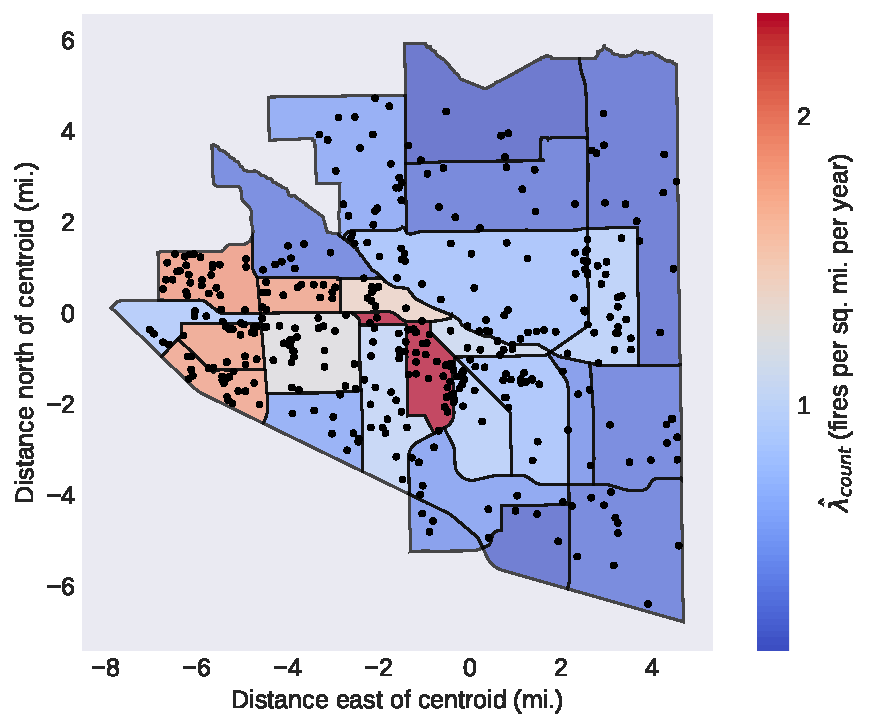
\includegraphics[width=.75\textwidth]{./figures/spatial_histogram.pdf}
\caption{A visual depiction of the naive count forecasting methodology for an example department. The black dot markers indicate the location of a residential fire that occurred during the six-year training interval, 2006-2011 (inclusive). The color corresponds to the fire count density rate estimated from this approach. Notice that large census tracts with few fires have the lowest density rate and small tracts with many fires have the highest density rate.}
\label{fig:spatial_histogram}
\end{figure}

\subsubsection{Kernel density estimation}
\label{sec:kde}
The second spatial model discussed in this paper is kernel density estimation (KDE), which is a statistical methodology for inferring a density distribution from a set of point observations. This is the framework commonly used to generate incident heatmaps. The major difference between this method and the one outlined in the previous section is that KDE results  a smoothed surface that does not arise from ``binning" the incidents into discrete areas such as the census tract boundaries. Instead, this density surface is generated by centering a kernel function on each point (i.e. residential fire location) in the training set. The density function can then be calculated at any location by summing the kernel functions of all past residential fires at that location. This process is described by equation \ref{eqn:kde}:

\begin{equation}
  \label{eqn:kde}
  \hat\lambda_{i}^\text{KDE}(\textbf{x}) = \frac{1}{n^{\text{train}}}\sum_{m=1}^{F_i}K_i(\textbf{x},\tilde{\textbf{x}}_{i,m})
\end{equation}

\noindent where $F_i$ is the total number of fires that occurred during the training interval, and $\tilde{\textbf{x}}_{i,m}$ is the location of the $m^{th}$ residential fire that occured during the training interval in the coverage area of department \textit{i}. Note that the subscript \textit{j} is not used here because $\hat\lambda_{i}^\text{KDE}(\textbf{x})$ does not depend on census tract geometries. $K_i(\textbf{x},\tilde{\textbf{x}}_{i,m})$ is a department-specific kernel function. The KDE predictions described in this paper were obtained using a two-dimensional isotropic Gaussian kernel, described in equation \ref{eqn:gaussian_kernel}:

\begin{equation}
  \label{eqn:gaussian_kernel}
  K_i(\textbf{x},\tilde{\textbf{x}}_{i,m}) = \frac{1}{2\pi b_{i}^2}exp\bigg(\frac{-d^2(\textbf{x},\tilde{\textbf{x}}_{i,m})}{2b_{i}^2}\bigg)
\end{equation}

\noindent where $d(\textbf{x},\tilde{\textbf{x}}_{i,m})= ||\textbf{x} - \tilde{\textbf{x}}_{i,m}||_2$, the euclidean distance between an arbitrary point \textbf{x} and $\tilde{\textbf{x}}_{i,m}$. $b_i$ is the department-specific bandwidth. Loosely speaking, it represents the length scale over which past fires elevate the estimated fire risk of surrounding areas. An important attribute of the kernel used in these analyses is that $\int_{\textbf{x} \in \textbf{R}^2}K_i(\textbf{x},\tilde{\textbf{x}}_{i,m})d\textbf{x} = 1$, and by extension, $n^{\text{train}}\int_{\textbf{x} \in \textbf{R}^2}\hat\lambda_{i}^\text{KDE}(\textbf{x}) d\textbf{x} = F_i$. In other words, the total kernel density is equal to the total number of fires that occurred during the training interval. In order to provide intuition for the reader, a simplified illustration of the KDE approach is provided in Figure \ref{fig:1dkde}.

\begin{figure}[htb] \centering
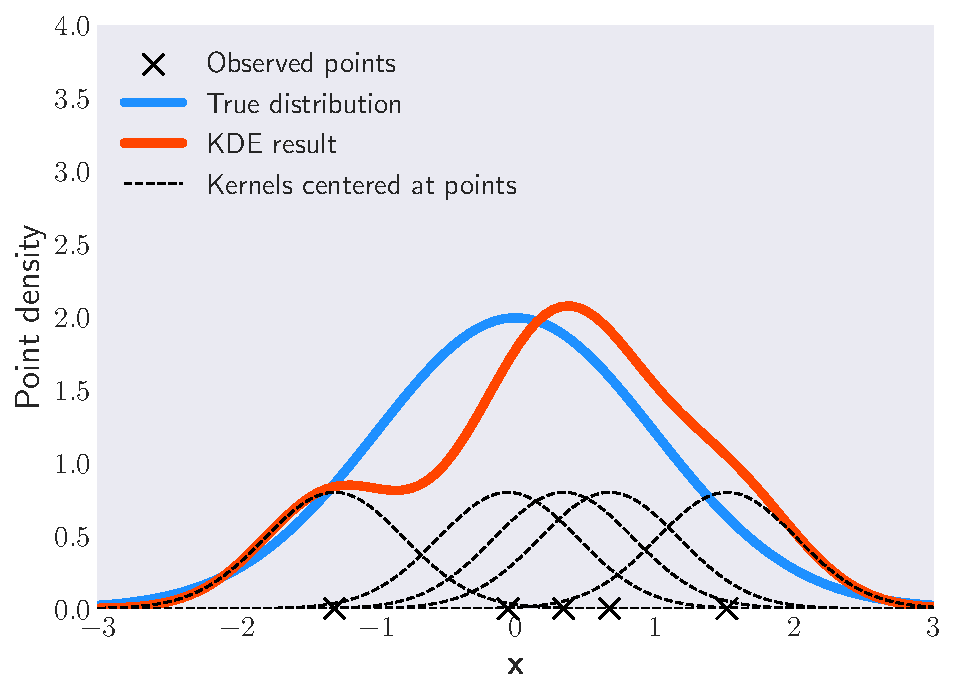
\includegraphics[width=.75\textwidth]{./figures/1dkde.pdf}
\caption{A simplified one-dimensional illustration of the KDE method. Although the locations of residential fires are defined in $\textbf{R}^2$, the use of a location coordinate defined in $\textbf{R}$ allows for an intuitive visualization. Five points (indicated by the ``X" markers) are drawn from a standard normal distribution, so that the true density function (the blue curve) is five times the standard normal probability distribution. The dashed black curves indicate Gaussian kernels centered on each point, and the red curve shows the KDE result, which is the sum of the kernels.}
\label{fig:1dkde}
\end{figure}

A key consideration for generating meaningful results from KDE is the selection of the bandwidth parameter, $b_i$. Selecting too small of a bandwidth results in density estimates that have highly localized peaks that correspond to the locations of past incidents; conversely, selecting too large of a bandwidth results in an overly smoothed density estimate that tends towards a uniform density profile as $b_i \rightarrow  \infty$. Figure \ref{fig:band_comparison} shows the effect of different bandwidth on the resulting KDE heatmaps along with the "optimized bandwidth" which is obtained through 5-fold cross validation. This technique randomly splits the training data into five groups of approximately equal size. Using a specific value for $b_i$, a KDE map is generated using the data from four of the five groups or folds. The algorithm then determines the likelihood of the the locations of the fires in the excluded fold using the map generated from incidents in the four remaining folds. This likelihood arises from the fact that $\frac{n^{\text{train}}}{F_i}\hat\lambda_{i}^\text{KDE}(\textbf{x})$ is actually an estimate of the probability density function for the location of a new fire. This process is then repeated so that each of the five folds are excluded, and 100 logarithmically spaced values of $b_i$ are evaluated over the interval $[0.01,10]$ miles and the bandwidth that generated KDE maps with the highest predictive accuracy is chosen as the optimal bandwidth, $b_{i}^{\text{opt}}$. This optimization process is described mathematically by equation \ref{eqn:fivefold}:

\begin{equation}
  \label{eqn:fivefold}
   b_{opt,i} = \argmax_{b_i} \prod_{k=1}^5 \prod_{m \in E_k}   \hat\lambda_{i,k}(\tilde{\textbf{x}}_m,b_i)
\end{equation}

\noindent where $\hat\lambda_{i,k}(\tilde{\textbf{x}}_m,b_i)$ is the KDE function that is generated using a bandwidth of $b_i$ and also excluding incidents in the k$^{th}$ fold, $E_k$. 

\begin{figure}[!ht]
       \begin{center}
  %
          \subfloat[$b_i=0.1$ mi]{%
              \label{fig:smallband} 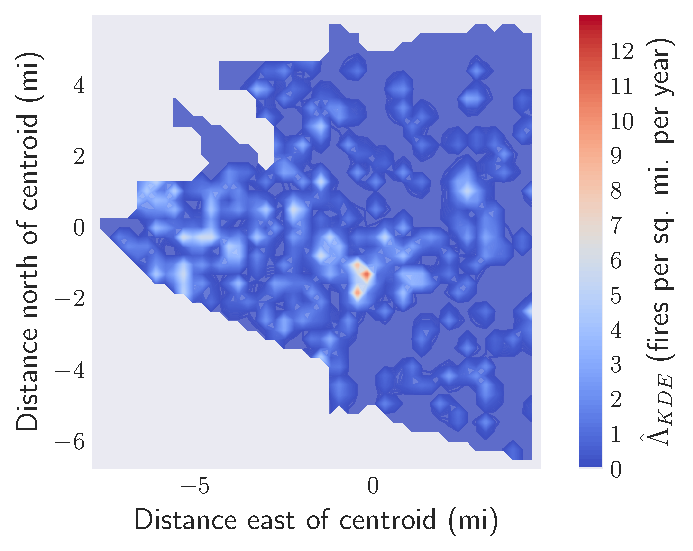
\includegraphics[width=.4\textwidth,keepaspectratio]{figures/small_band.pdf}
          }%
          \subfloat[$b_i= 1.0$ mi]{%
             \label{fig:largeband} 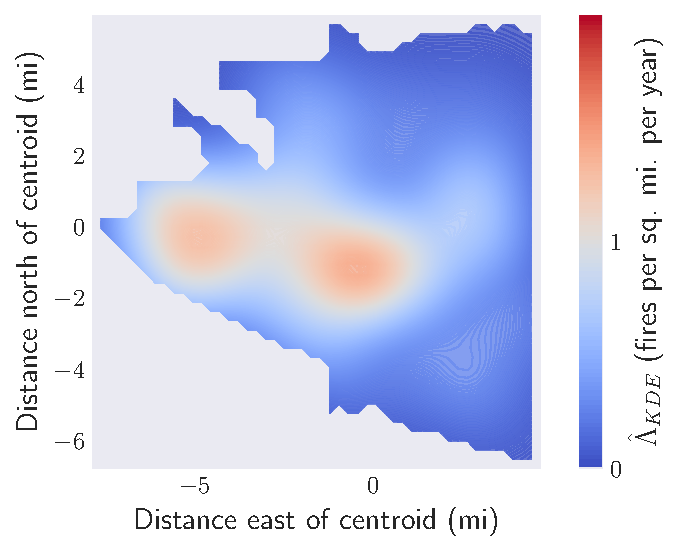
\includegraphics[width=.4\textwidth ,keepaspectratio]{figures/large_band.pdf}
          }\\ % 
            \subfloat[$b_i=b_{i}^{\text{opt}}=0.43$ mi]{%
             \label{fig:optband} 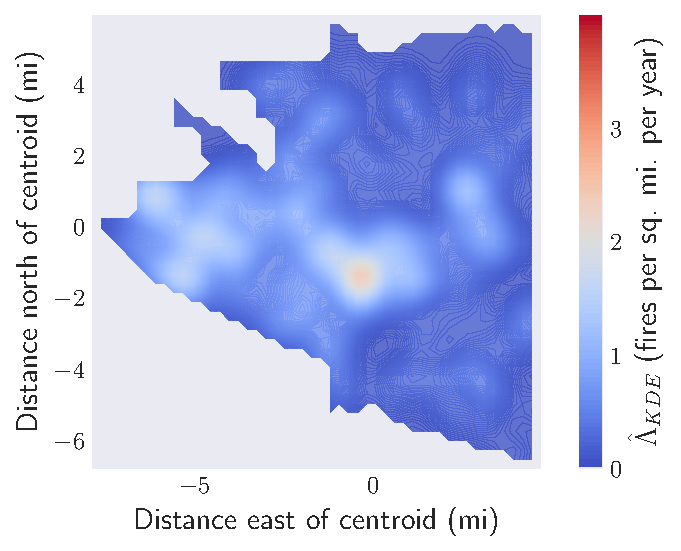
\includegraphics[width=.4\textwidth,keepaspectratio]{figures/correct_band.pdf}
          } % ------- End of the first row ----------------------%
      \end{center}
      \caption{ Visual depiction of the effect of different bandwidth values for heatmaps generated from KDE. The bandwidth is too small in \protect\subref{fig:smallband}, which is apparent from the many localized ``hotspots."  Conversely, the bandwidth is too large in \protect\subref{fig:largeband}, and the result is an overly smoothed heatmap. \protect\subref{fig:optband} shows the heatmap with the optimized bandwidth.}
     \label{fig:band_comparison}
  \end{figure}
  
 As previously indicated, the central idea of KDE is that proximity to past fires elevates the probability of future fires, and $b_{i}^{\text{opt}}$ is the distance that best specifies this proximity\footnote{Approximately 95\% of the kernel density from an incident is located within $2b_i$ of the incident location.} for predicting the locations of ``out of sample" fires. This means that the results obtained from the bandwidth optimizations give insight into the distances over which fire risk factors vary within the coverage areas of the departments in the dataset. Figure \ref{fig:bhist} shows that these distances vary significantly across departments, though $b_{i}^{\text{opt}}$ was between 0.1 and 0.4 miles for most departments. Furthermore, Figure \ref{fig:popband} reveals a negative correlation between $b_{i}^{\text{opt}}$ that explains some of the variation of $b_{i}^{\text{opt}}$ across the departments in the dataset. This result implies that residential fire risk factors spatially vary more significantly in communities with higher population densities than those with lower population densities. For example, knowledge of residential fires that occurred 0.75 miles away from a specific housing unit may elevate the probability of that unit experiencing a fire in regions of low population density, but less so in regions of high population density.

\begin{figure}[!ht]
       \begin{center}
  %
          \subfloat[Histogram of optimized bandwidths]{%
              \label{fig:bhist} 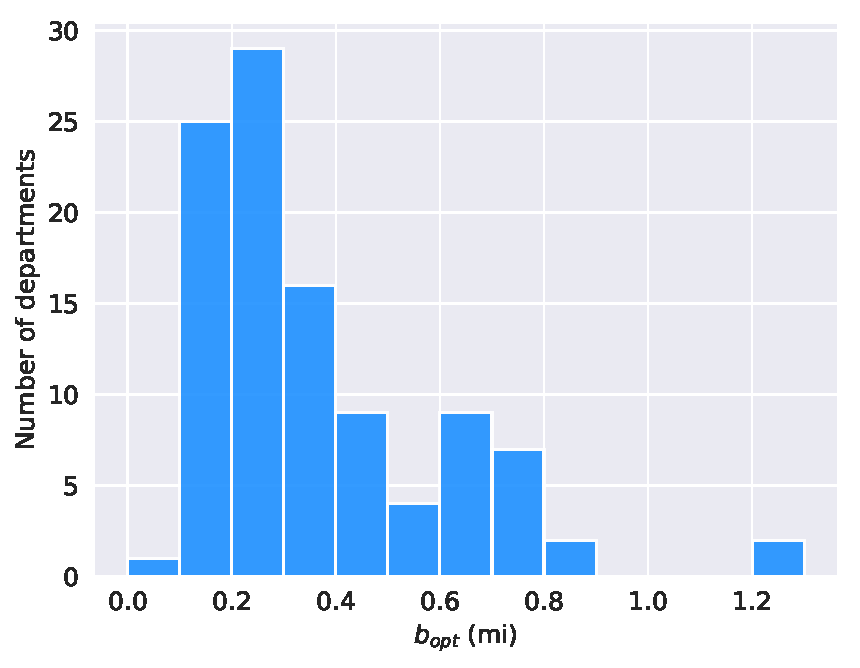
\includegraphics[width=.4\textwidth,keepaspectratio]{figures/optimal_band_dist.pdf}
          }%
          \subfloat[Scatterplot of optimized bandwidths vs. average department population density]{%
             \label{fig:popband} 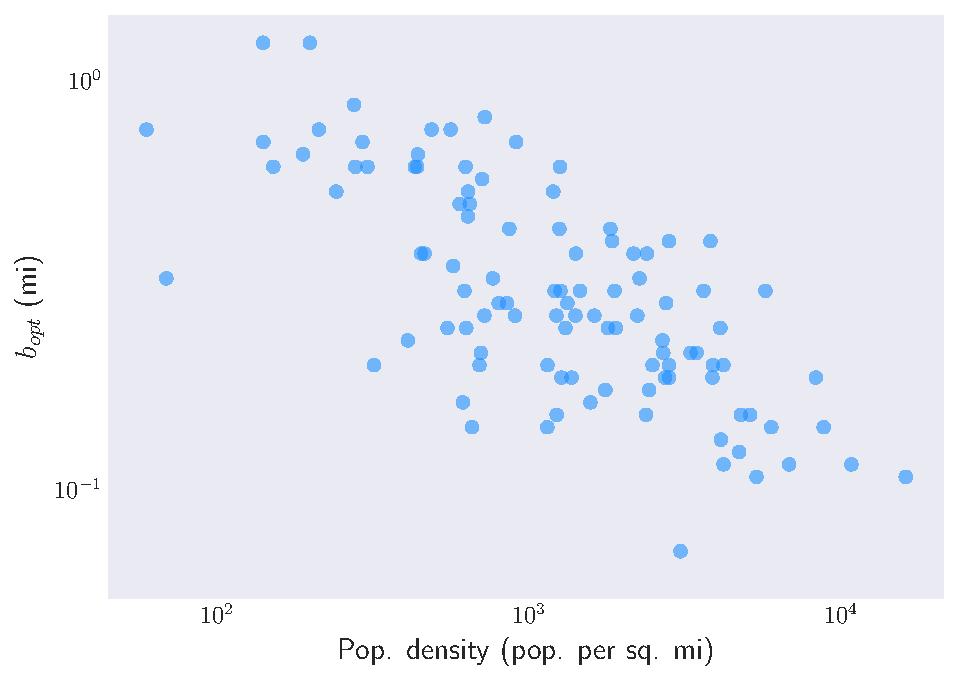
\includegraphics[width=.4\textwidth,keepaspectratio]{figures/boptvspopdensity.pdf}
          } % 
           % ------- End of the first row ----------------------%
      \end{center}
      \caption{\protect\subref{fig:bhist} shows the variation of the optimized bandwidth across departments in the dataset, and the negative correlation apparent in \protect\subref{fig:popband} shows that this variation is at least partially explained by the variation in population density across departments.}
     \label{fig:band_optimization}
  \end{figure}
  
  Calculating $b_{i}^{\text{opt}}$ for each department allows for the determination of $\hat\lambda_{i}^\text{KDE}(\textbf{x})$ according to equation \ref{eqn:kde}. The KDE estimate for the number of fires that occur during the test interval can then be obtained from equation \ref{eqn:rate_description}. However, because $\hat\lambda_{i}^\text{KDE}(\textbf{x})$ does not have an analytical form, the estimate is generated by evaluating it at a set of 100 by 100 evenly spaced grid points within each census tract and then performing a numerical integration. Note that this generates different estimates of  $\Lambda_{i,j}$ than using the spatial histogram approach because the kernel densities from individual fire incidents ``spill out" across census tract boundaries. In fact, The spatial histogram approach can be viewed as a special case of the KDE approach where $b_i \rightarrow 0$, which makes the kernels analagous to a set of Dirac delta functions in which the entire density is located at a point, but it still integrates to one.
  
 

  \subsection{Utilizing demographic and structural information}
  In contrast to the models presented in the previous section, the focus of this section is to utilize only the socio-demographic and structural information from the American Community Survey 5-year summary file (ACS5). In this section, the fire incident location data is used only to assign each incident to a census tract. After these assignments, the ACS5 data is the sole basis of the training features. This means that the location of census tracts relative to other census tracts is not incorporated into the model described in this section.

  \subsubsection{Feature visualization}
  Before desribing the model that utilizes ACS5 data, it is worth understanding the underlying relationships between the fire rates in census tracts and their structural and socio-demographic profiles. Perhaps the most intuitive starting point is the recognition that residential fires occur where people live, so it is reasonable to expect a positive relationship between the rate of fires experienced by a census tract and its population. The authors found that normalizing these quantities by the census tract area improves the clarity of the relationship, which is shown in Figure \ref{fig:pop_relation}. It also allows for the delineation between urban and rural communities; as a rule of thumb, the Census Bureau   \cite{ratcliffe2016defining} uses a population density of 1,000 pop. per. sq. mile as a guideline for the cutoff between urban and rural for census blocks. Although the dataset is comprised of census tracts rather than blocks and this criterion serves as one component of the urban/rural designation, it still provides intuition for the separation between rural and urban communities, and as a result is chosen as the separating line in the figures. The relationship is fairly linear on a log-log scale, which is the first trend that can be used to inform a predictive model.
    
     \begin{figure}[htb] \centering
    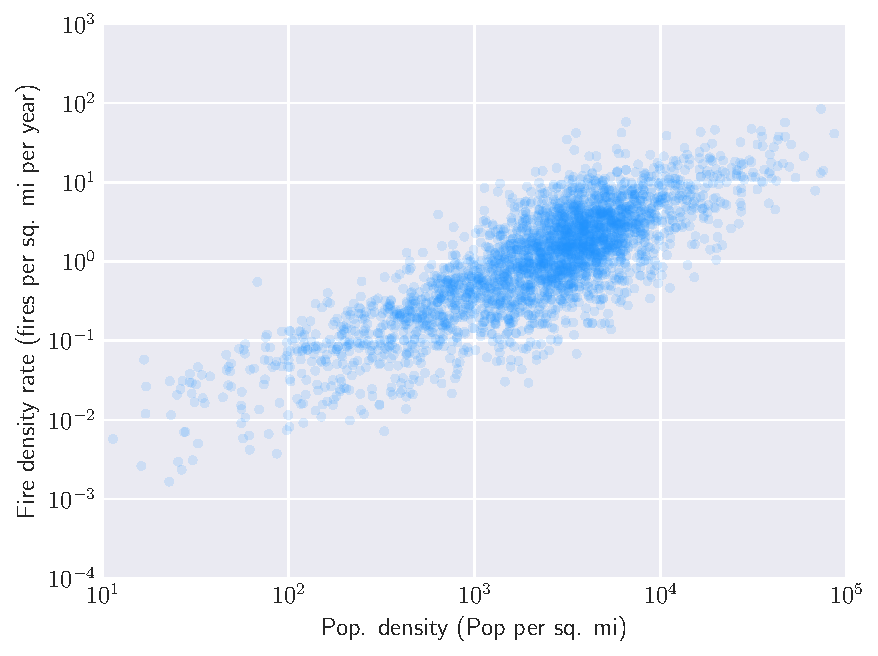
\includegraphics[width=.75\textwidth]{figures/pop_relation.pdf}
    \caption{A scatterplot of the observed fire count density rate   during the training interval vs. population density for all 3,009 census tracts in the dataset. }
    \label{fig:pop_relation}
    \end{figure}
  
  In light of the linear relationship shown in Figure \ref{fig:pop_relation}, the effects of other socio-demographic factors that influence fire risk can be understood in terms of upward or downward ``shifts" to the approximately linear cloud of points representing census tracts. This also can be viewed as changes in the fire rate per person. This is shown in Figure \ref{fig:sociodemographic}.
  
  \begin{figure}[!ht]
       \begin{center}
  %
          \subfloat[Median income]{%
              \label{fig:median_income} 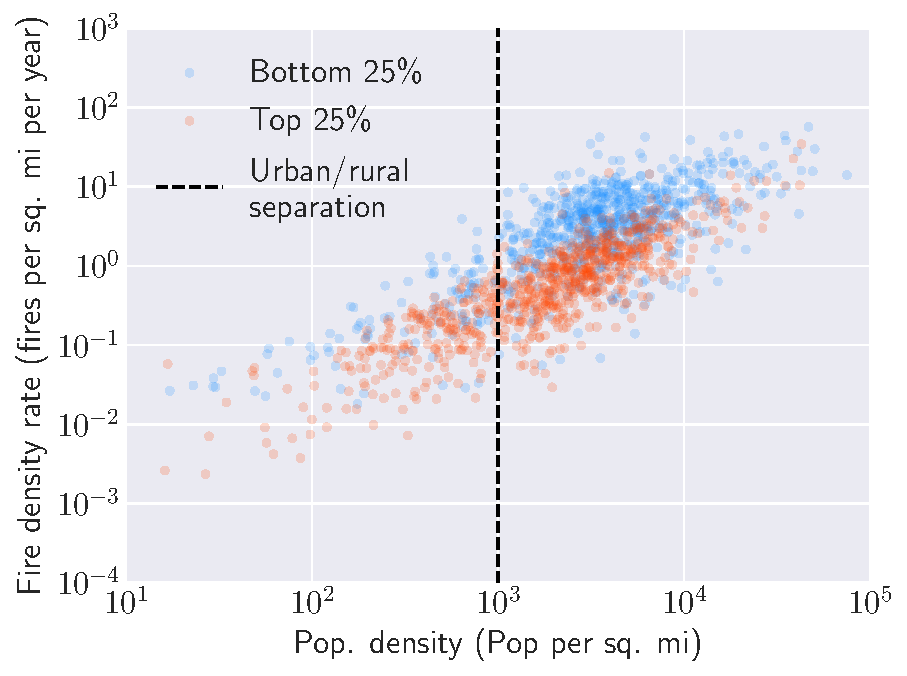
\includegraphics[width=.4\textwidth,keepaspectratio]{figures/median_income.pdf}
          }%
          \subfloat[Fraction of population holding college degrees]{%
             \label{fig:frac_degree} 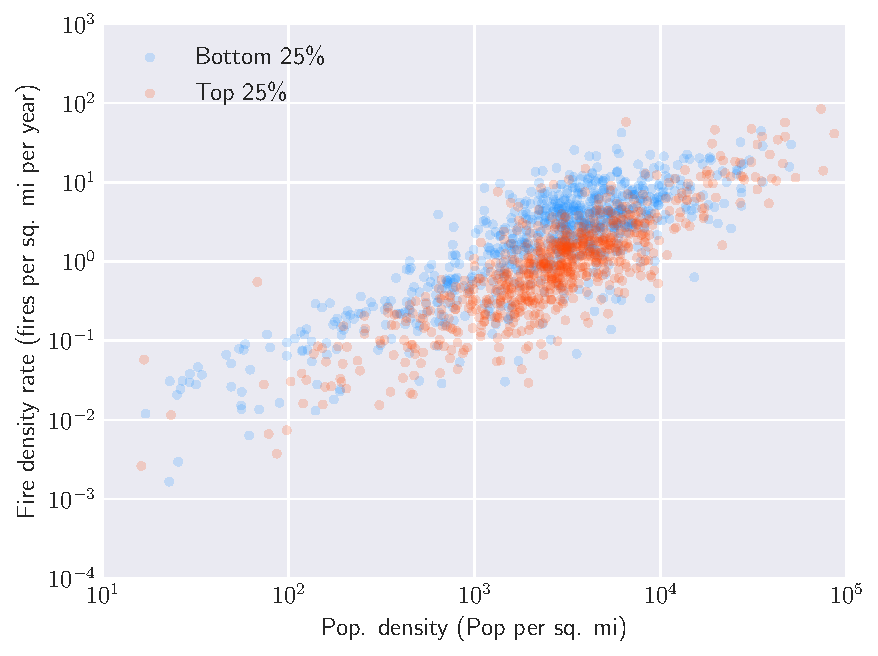
\includegraphics[width=.4\textwidth,keepaspectratio]{figures/frac_degree.pdf}
          }\\ % 
            \subfloat[Fraction of population that is Black]{%
             \label{fig:frac_black} 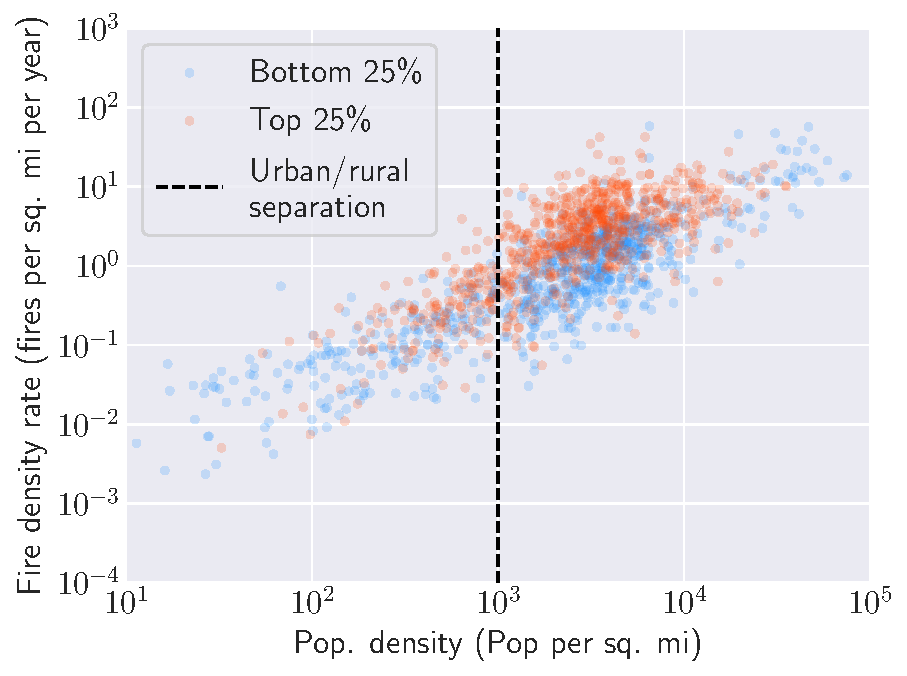
\includegraphics[width=.4\textwidth,keepaspectratio]{figures/frac_black.pdf}
          }
            \subfloat[Fraction of population that is White]{%
             \label{fig:frac_white} 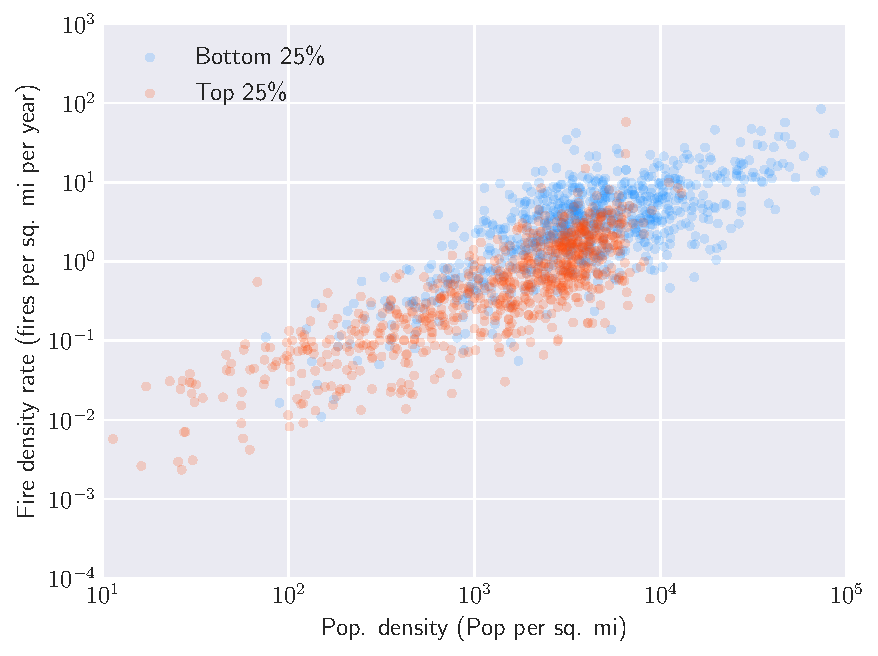
\includegraphics[width=.4\textwidth,keepaspectratio]{figures/frac_white.pdf}
          }\\
            \subfloat[Fraction of population that is Asian]{%
             \label{fig:frac_asian} 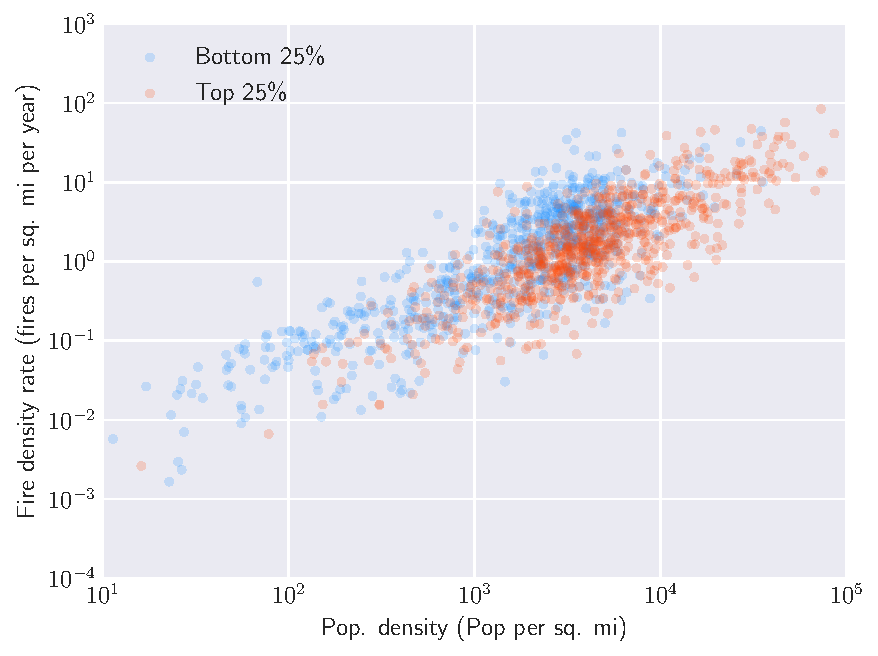
\includegraphics[width=.4\textwidth,keepaspectratio]{figures/frac_asian.pdf}
          }
            \subfloat[Fraction of population that is Hispanic]{%
             \label{fig:frac_hispanic} 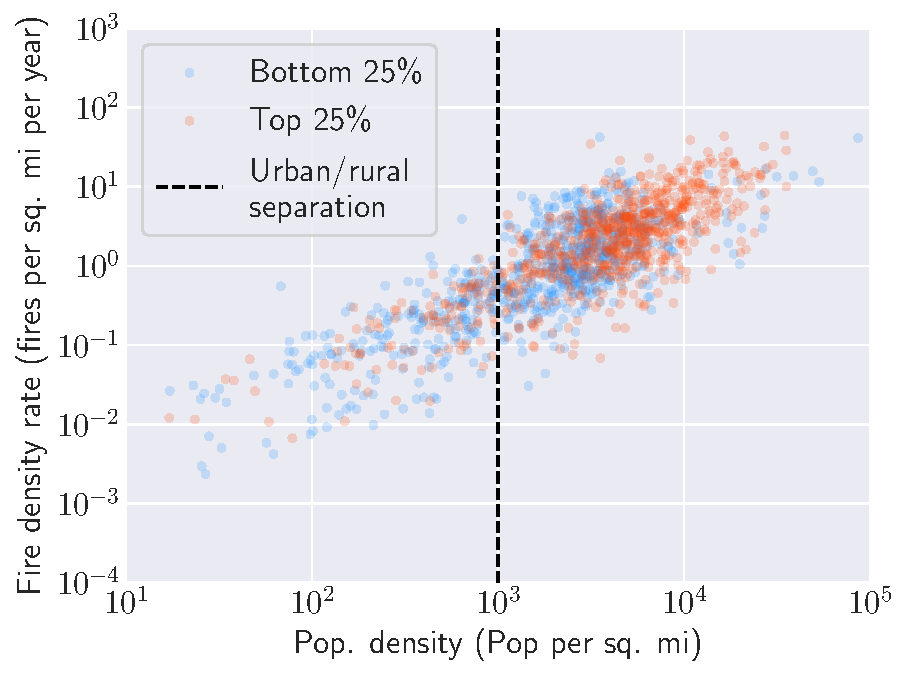
\includegraphics[width=.4\textwidth,keepaspectratio]{figures/frac_hispanic.pdf}
          }
      \end{center}
      \caption{Scatterplot of observed fire density rates during the training interval as a function of population density for census tracts in the top quartile (red) and bottom quartile (blue) of the specified sociodemographic quantities. For example, in \protect\subref{fig:median_income}, the red dots represent census tracts with median incomes in the top 25\% of all tracts in the dataset. Conversely, the blue dots represent census tracts with median incomes in the bottom 25\% of all census tracts in the dataset.}
     \label{fig:sociodemographic}
  \end{figure}
 
 
 These visualizations give insight into the populations who are most at risk for residential fires. Figures \ref{fig:median_income} and \ref{fig:frac_degree} show the expected result that census tracts with educated and high earning populations experience fires at a lower rate than those with low income or less educated populations. Interestingly, the relationship within the top and bottom quartiles of these quantities still appears linear, but the effect of increased socioeconomic status appears to shift the linear trend downward in the log-log plots. The effects of the racial and ethnic compositions shown in Figures \ref{fig:frac_black}-\ref{fig:frac_hispanic} show similar trends, which is likely due to the fact that these quantities are correlated with the socioeconomic factors shown in Figures \ref{fig:median_income} and \ref{fig:frac_degree}. 
 
Figure \ref{fig:building age} gives insight into the effect of building age on the fire frequency. The visualizations show the expected result that residential fires are more likely to occur in older buildings than newer ones. Interestingly, the census tracts with the highest fractions of buildings built before 1950 appear mostly in urbanized areas in the dataset, yet the cloud of points comprised of these census tracts appears to lie slightly above that comprised of the census tracts with fractions of buildings built before 1950 in the bottom quartile. Conversely, census tracts with a large fraction of housing units built more recently than 1990 have lower population densities and a slightly lower fire risk per person as well.

   \begin{figure}[!ht]
       \begin{center}
  %
          \subfloat[Fraction of housing units built before 1950]{%
              \label{fig:frac_1950} 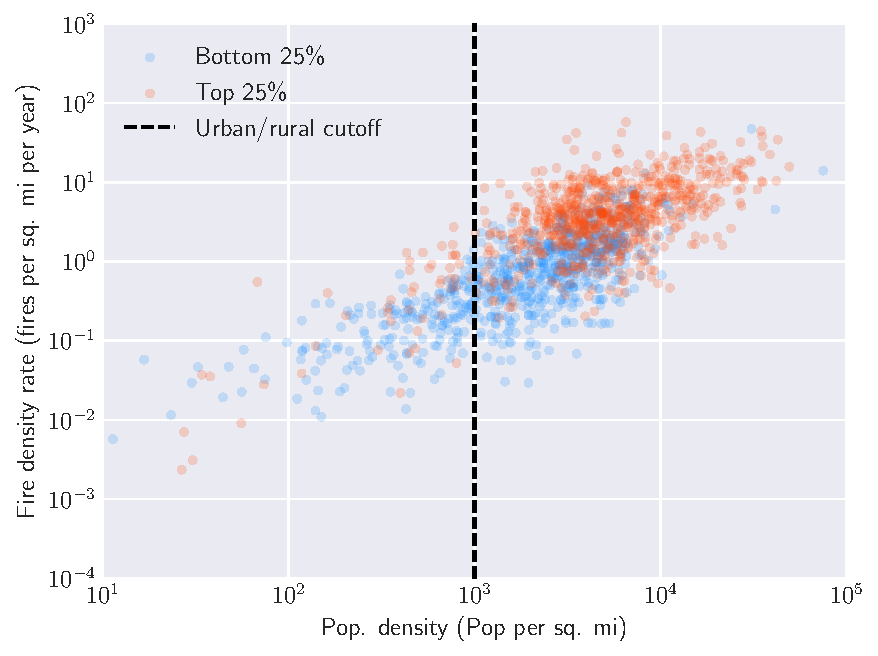
\includegraphics[width=.4\textwidth,keepaspectratio]{figures/frac_1950.pdf}
          }%
          \subfloat[Fraction of housing units built between 1950 and 1969]{%
             \label{fig:frac1950_1969} 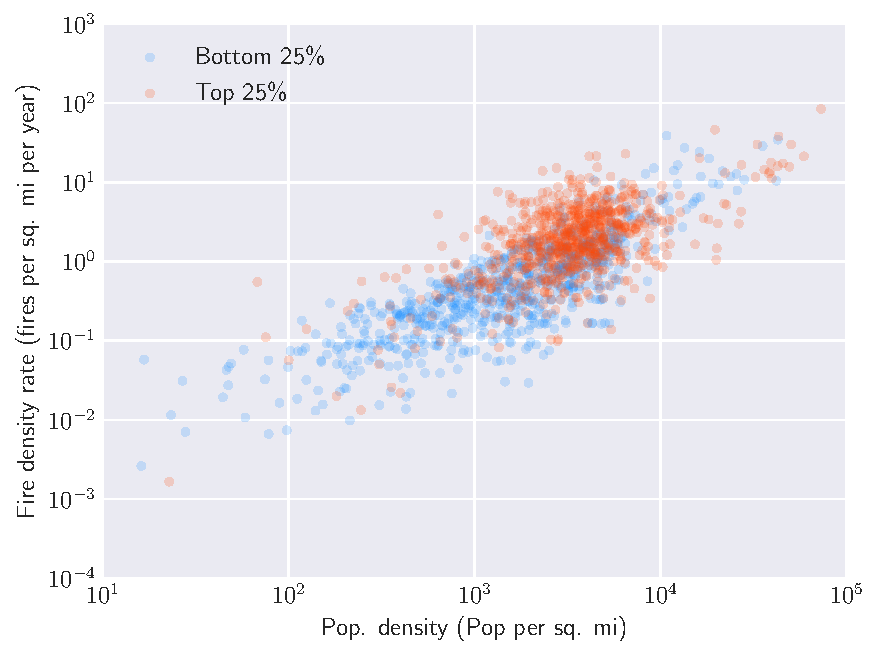
\includegraphics[width=.4\textwidth,keepaspectratio]{figures/frac_1950_1969.pdf}
          }\\ % 
            \subfloat[Fraction of housing units built between \newline 1970 and 1989]{%
             \label{fig:frac_1970_1989} 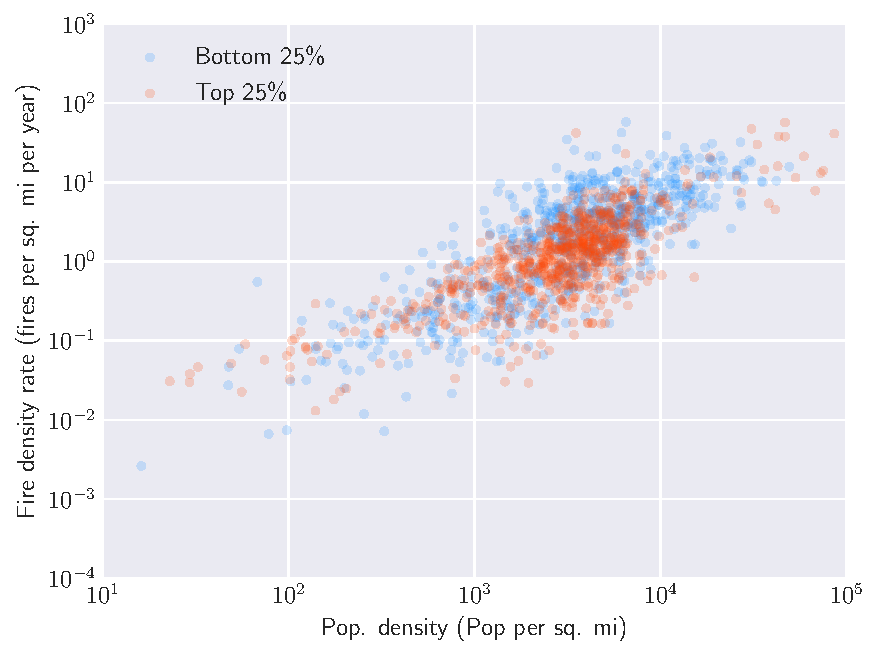
\includegraphics[width=.4\textwidth,keepaspectratio]{figures/frac_1970_1989.pdf}
          }
            \subfloat[Fraction of housing units built in 1990 or later]{%
             \label{fig:frac_1990} 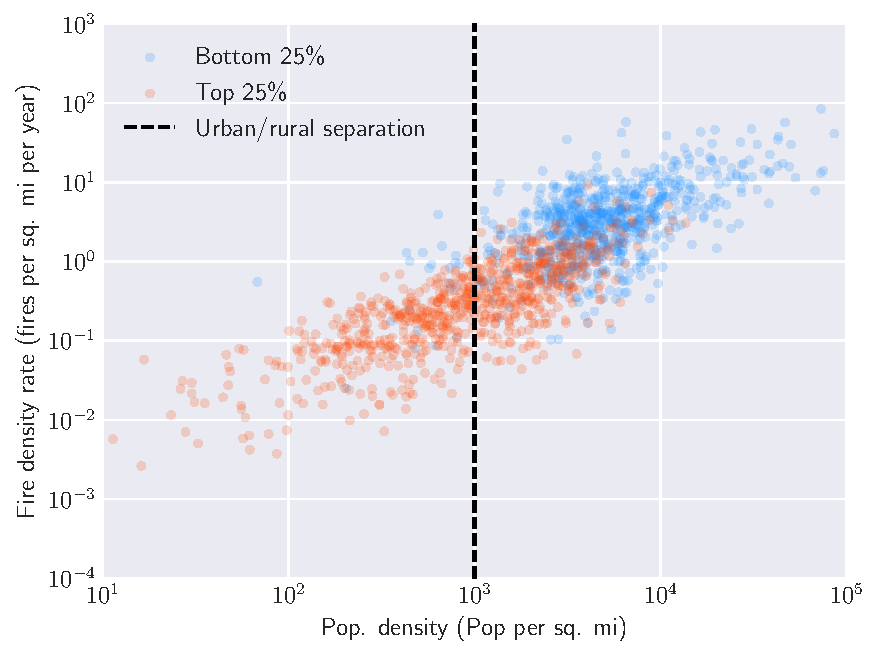
\includegraphics[width=.4\textwidth,keepaspectratio]{figures/frac_1990.pdf}
          }\\
          
      \end{center}
      \caption{Scatterplot of observed fire density rates ($\hat\Lambda^{\text{count}}$) during the training interval as a function of population density for census tracts in the top quartile (red) and bottom quartile (blue) of the specified quantity relating to structure age. For example, in \protect\subref{fig:frac_1950}, the red dots represent census tracts with fractions of housing units built before 1950 in the top 25\% of all tracts in the dataset. Conversely, the blue dots represent census tracts with fractions of housing units built before 1950 in the bottom 25\% of all census tracts in the dataset.}
     \label{fig:building age}
  \end{figure}
 
    Lastly, Figure \ref{fig:occupancy} gives insight into the effect of different occupancy characteristics on residential fire risk. Again, the expected trends appear- the fire risk appears to be greater in census tracts with higher fractions of renter-occupied housing compared to owner-occupied housing. Also, the differences in these features is correlated with population density with the top quartile of renter-occupied census tracts are mostly urbanized. Figure \ref{fig:frac_vacant} indicates that large fractions of vacant housing also appears to elevate the residential fire risk per person, but the top quartile appears to have more variability in the fire risk per person than the bottom quartile. This finding is consistient with the work of Schachterle et al. \cite{schachterle2012proximity}, who found that proximity to vacant housing increased fire risk in Baltimore, Maryland.  Not surprisingly, census tracts with large fractions of single-unit housing follows similar trends as those with high fractions of owner occupied units. 
 
   \begin{figure}[!ht]
       \begin{center}
  %
          \subfloat[Fraction of housing units occupied \newline by a renter]{%
              \label{fig:frac_rented} 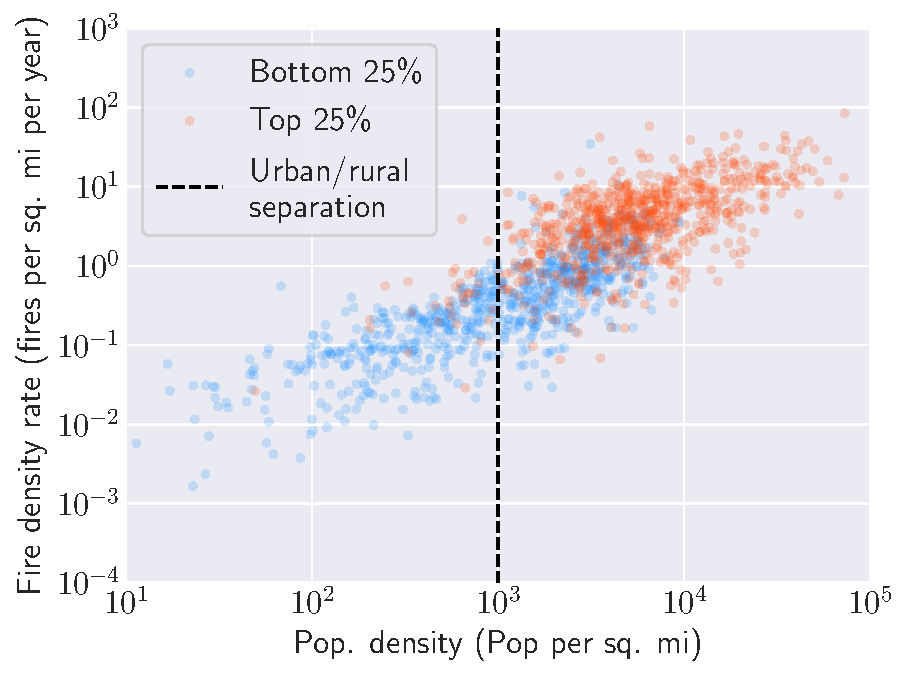
\includegraphics[width=.4\textwidth,keepaspectratio]{figures/frac_rented.pdf}
          }%
          \subfloat[Fraction of housing units occupied by the owner]{%
             \label{fig:frac_owner} 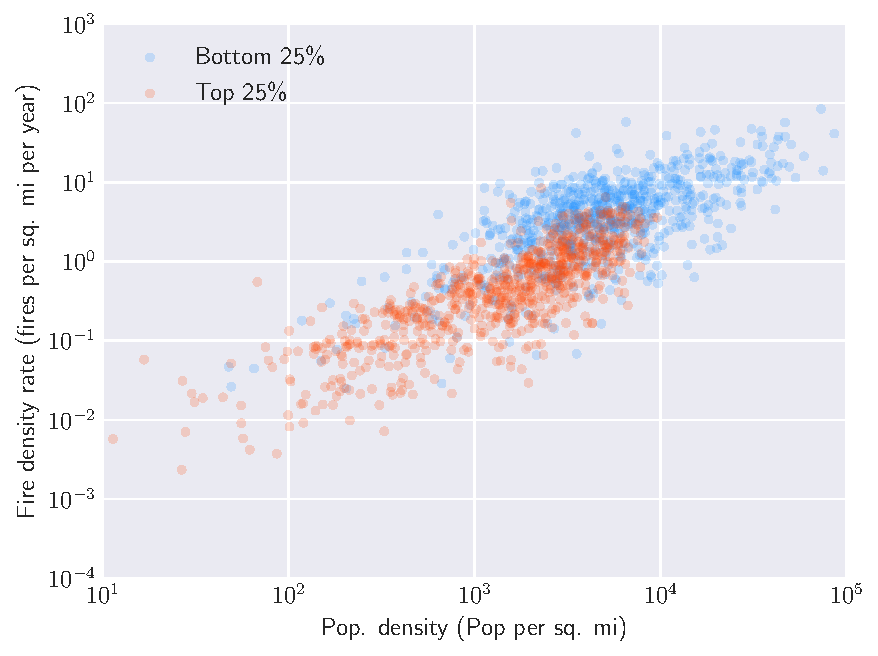
\includegraphics[width=.4\textwidth,keepaspectratio]{figures/frac_owner.pdf}
          }\\ %           
          \subfloat[Fraction of housing units that are vacant ]{%
             \label{fig:frac_vacant} 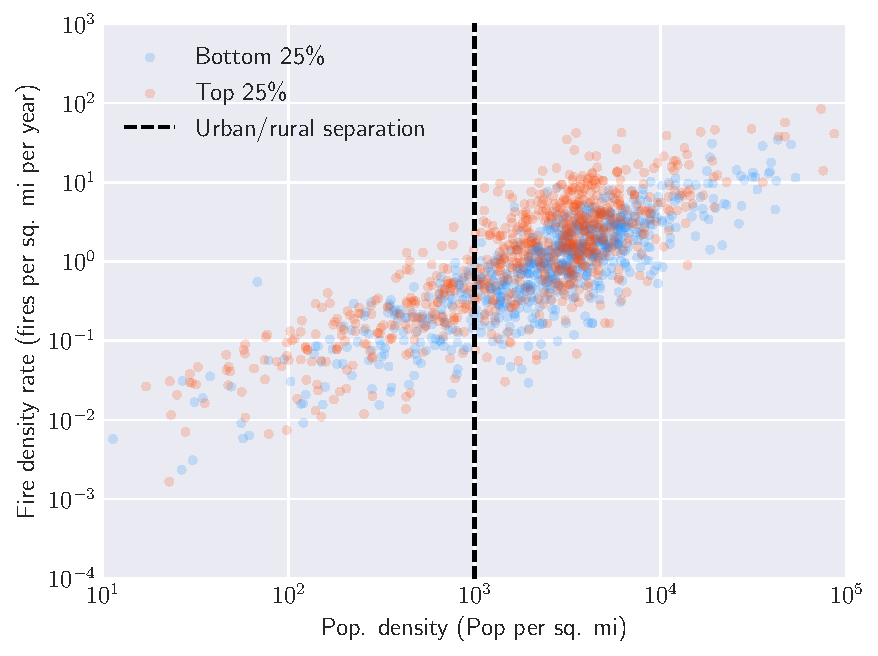
\includegraphics[width=.4\textwidth,keepaspectratio]{figures/frac_vacant.pdf}
          } % 
            \subfloat[Fraction of housing units that are single (not apartments)]{%
             \label{fig:frac_1_unit} 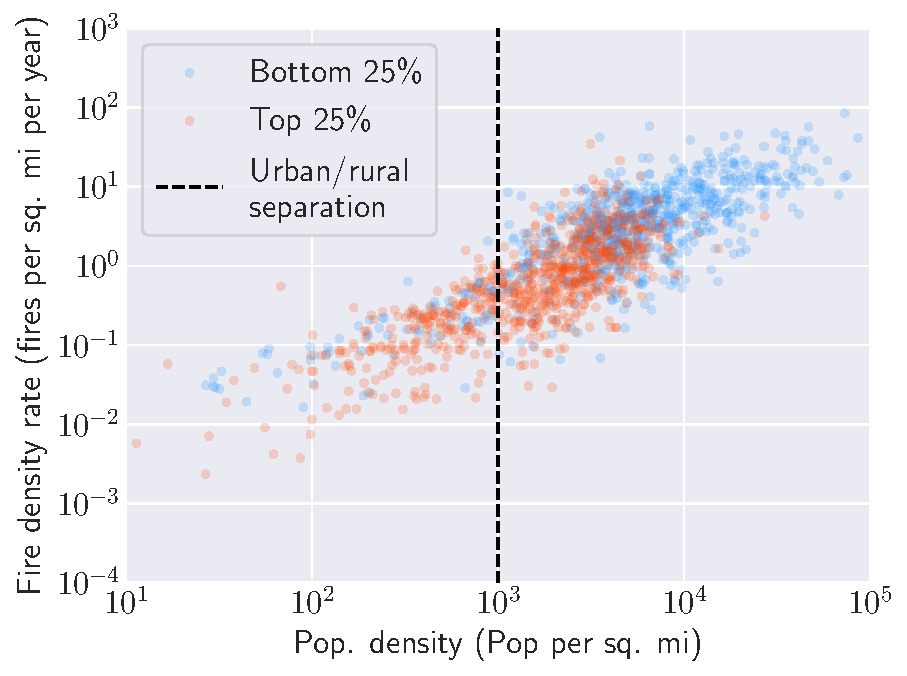
\includegraphics[width=.4\textwidth,keepaspectratio]{figures/frac_1_unit.pdf}
          }
      \end{center}
      \caption{Scatterplot of observed fire density rates ($\hat\Lambda^{\text{count}}$) during the training interval as a function of population density for census tracts in the top quartile (red) and bottom quartile (blue) of the specified quantity relating to occupancy. For example, in \protect\subref{fig:frac_rented}, the red dots represent census tracts with fractions of housing units occupied by a renter in the top 25\% of all tracts in the dataset. Conversely, the blue dots represent census tracts with fractions of housing units occupied by a renter in the bottom 25\% of all census tracts in the dataset.}
     \label{fig:occupancy}
  \end{figure}
 
 
 \clearpage
  \subsubsection{Dimensionality reduction}
    In order to reduce the dimensionality of the training dataset, a principal components analysis (PCA) was conducted using the machine learning libarary SciKitLearn \cite{pedregosa2011scikit}. PCA is a statistical technique that utilizes correlations between input variables to reduce the dimensionality of the dataset. This is done by projecting the input data into a new space where certain dimensions can be disregarded while still retaining most of the variation of the original dataset. The projection vectors are the eigenvectors of the covariance matrix of feature variables and the transformed features are linearly uncorrelated. A simple example of this technique is illustrated in \ref{fig:pca}.
  
    \begin{figure}[!htb]
       \begin{center}
  %
          \subfloat[Original data]{%
              \label{fig:pca_raw} 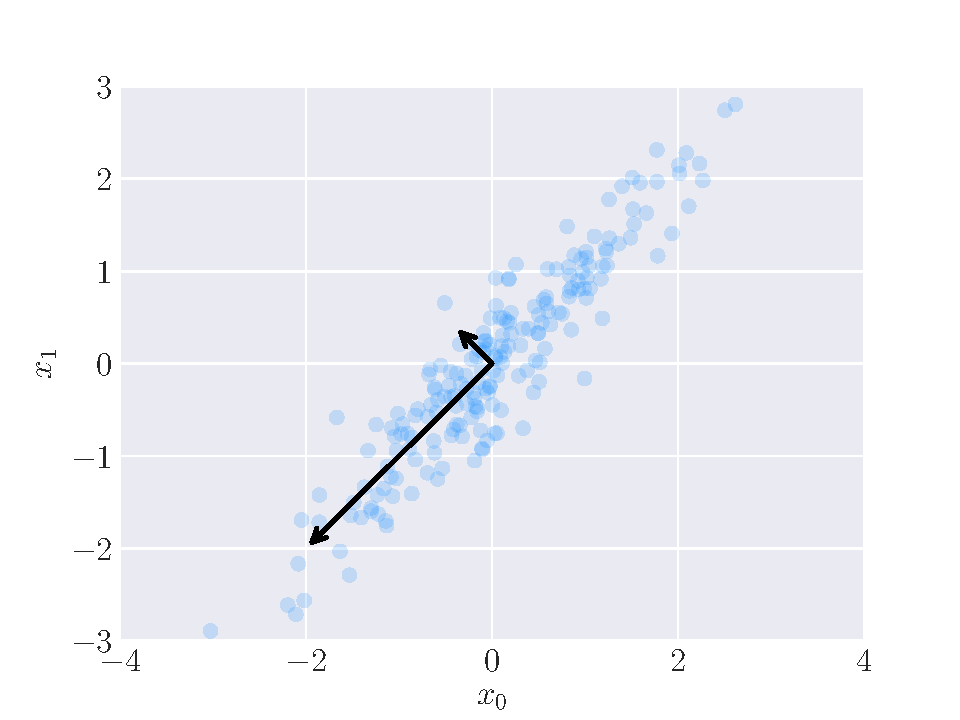
\includegraphics[width=.4\textwidth,keepaspectratio]{figures/pca_raw.pdf}
          }%
          \subfloat[PCA transformed data]{%
             \label{fig:pca_projected} 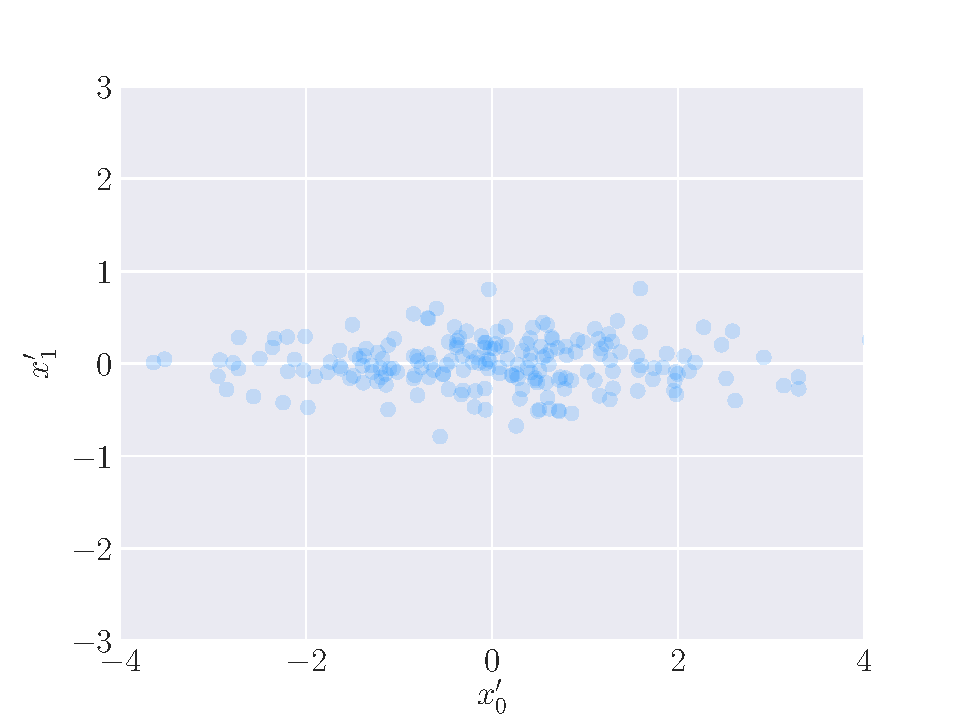
\includegraphics[width=.4\textwidth,keepaspectratio]{figures/pca_projected.pdf}
          } %           
      \end{center}
      \caption{A simple example of the PCA technique on synthetic data. Figure \protect\ref{fig:pca_raw} shows the raw data in two input dimensions, $x_0$ and $x_1$, which are visibly correlated. The principal component vectors are also shown, which are the eigenvectors of the covariance matrix. These vectors are then used to project (rotate) the data into the space defined by the variables $x_0^\prime$, and $x_1^\prime$, which are uncorrelated. In this new space, one variable, $x_0^\prime$ explains over 96\% of the total variance, allowing for the reduction to one dimension without significant loss of information.}
     \label{fig:pca}
  \end{figure}
  
  Using PCA, the eight sociodemographic features were reduced to five that explained 91\% of the variance, and the six structural features were reduced to four that also explained 91\% of the variance. This allowed for the generation of an $N_i$x10 training feature matrix for each department, $\textbf{X}_i$. Note that the feature matrix contains a column of ones for the intercept in addition to the 9 feature variables that were generated from PCA. Note that the population density is also excluded from $\textbf{X}_i$. 
  
  
  
  \clearpage
  
 \subsection{A hierarchical Bayesian Poisson regression model}
 \label{sec:bayes}
 The feature visualizations motivated the use of a Poisson regression model according to the following form:
 
 \begin{equation}
  \label{eqn:poisson_regression}
  \underbrace{log(\hat\lambda^{\text{HPR}}_{i,j})}_{\text{I}} =   \underbrace{\eta\gamma_{i,j}}_{\text{II}} + \underbrace{\textbf{X}_{i,j}\beta_{i}}_{\text{III}}
\end{equation}

\noindent where $\hat\lambda^{\text{HPR}}_{i,j}$ is the area-averaged intensity function value for census tract $j$ in department $i$ such that $\hat\lambda^{\text{HPR}}_{i,j}=\hat\lambda^{\text{HPR}}_{i,j}A_{i,j}$. The ``HPR" superscript indicates that the estimate is generated using the hierarchical Poisson regression model. $\beta_i \in \textbf{R}^{10}$ is a vector of regression coefficients that quantify the effects of the PCA feature variables on the rate of fires in each census tract. Note that the subscript $i$ indicates that the feature effects can vary between departments. $\gamma_{i,j}$ is the natural logarithm of the population density for census tract $i,j$, and $\eta$ is the global population density effect. The relationship between terms I and II is motivated by the linear relationship in log-log space between the fire count density rate and the population density shown in \ref{fig:pop_relation}. Term III has the effect of shifting the linear relationship between terms I and II up or down, as shown by the feature visualizations in Figures \ref{fig:sociodemographic}-\ref{fig:occupancy}. Unlike traditional regressions in which one would minimize a cost function such as the sum of squared errors, a Bayesian regression is used, which yields posterior distributions of $\beta$ and $\eta$ given the observed fire counts during the training interval, and priors placed on $\beta$ and $\eta$. The likelihood is a Poisson distribution, shown in equation \ref{eqn:likelihood}.

 \begin{equation}
  \label{eqn:likelihood}
  P(f^{\text{train}}_{i,j}|\beta_i, \eta) = \frac{(n^{\text{train}}\lambda^{\text{HPR}}_{i,j})^{f^{\text{train}}_{i,j}} exp(-n^{\text{train}}\lambda^{\text{HPR}}_{i,j})}{f^{\text{train}}_{i,j}!}
\end{equation}

Note that the use of a Poisson likelihood is used because Figure \ref{fig:dispersion} in Appendix \ref{dispersion} indicates that the fire counts are not significantly overdispersed for most departments. This refers to the restriction of a Poisson distribution that the variance must equal the mean. In many cases, the variance is much greater than the mean (overdispersed), which justifies the use of other distributions to quantify the likelihood for count data such as the negative binomial distribution. \noindent An uninformed normal prior is placed on $\eta$ with mean zero and an arbitrarily large variance of 20:

 \begin{equation}
  \label{eqn:eta_prior}
  \eta \sim N(0,20)
\end{equation}

\noindent Note that the variance of 20 is very large because the regression is done in log space. Also, These priors are standard choices in the literature on Bayesian hierarchical modeling, and are recommended by Gelman (2006) \cite{gelman2006prior} for situations when there is little or no subjective prior information available about the regression coefficients. At this point, one could similarly place uninformed priors on the components of $\beta_i$, but this approach is limited in that the model can only learn from the incident data from department $i$ in order to estimate $\beta_i$. To circumvent this issue, the model is made \textit{hierarchical}, which allows the model to learn from data across all departments while still producing heterogeneous estimates of $\beta_i$. This is done by making the parameters of the prior distribution of $\beta_i$ also random variables, that are also learned from the data:

 \begin{equation}
  \label{eqn:beta_prior}
  \beta_i \sim N\big(\mu,diag(\sigma^2)\big)
\end{equation}

\noindent where $\mu \in \textbf{R}^{10}$ and $\sigma^2 \in \textbf{R}^{10}$ are vectors of the means and variances of the effects of each of the 9 PCA features (plus an intercept) across departments. Finally, uninformed priors are placed on $\mu$ and $\sigma^2$:

 \begin{equation}
  \label{eqn:mu_prior}
  \mu \sim N\big(0,20I\big)
\end{equation}

 \begin{equation}
  \label{eqn:sigma2_prior}
  \sigma^2 \sim HalfFlat
\end{equation}

\noindent where $HalfFlat$ denotes an improper prior defined over the positive reals and $I$ is an 10x10 identity matrix.

Using the above model specification, the posterior distributions for $\eta, \beta, \mu$, and $\sigma^2$ are estimated using a No-U-Turn sampler \cite{hoffman2014no} using the Python package PyMC3 \cite{salvatier2016probabilistic}. Rather than generating an analytical expression for the posterior distributions, the result is a set of traces that contain draws from an approximations of the posterior distributions. Four chains were generated each with 5,000 iterations with a burn-in period of 1,000 draws to allow for the chains to converge. The samples from the four chains were then pooled together, which resulted in 4x(5,000-1,000) = 16,000 samples. Each sample consists of a draw of $\eta$ and draws of $\beta_i$ for all i. Thus, an estimate of $\hat\Lambda_{i,j}$ using equation \ref{eqn:poisson_regression} can be evaluated for each sample, resulting in 16,000 draws from an approximation of the posterior of $\hat\Lambda^{\text{HPR}}_{i,j}$. The mean of these draws is then used to evaluate $\hat{f}^{\text{test}}_{i,j}$ using equation \ref{eqn:rate_integral}.



  \subsection{Combining spatial, structural, and demographic information} 
  A spatial component can be incorporated into the Poisson regression model described in section \ref{sec:bayes} by performing kernel smoothing on the residuals, $\varepsilon_{i,j}$, of the regression predictions defined in log space according to equation \ref{eqn:log_res}:
  
    \begin{equation}
    \label{eqn:log_res}
    \varepsilon_{i,j} = log(\hat\lambda^{\text{count}}_{i,j})- log(\hat\lambda^{\text{HPR}}_{i,j}) 
    \end{equation}

\noindent where $\hat\lambda^{\text{HPR}}_{i,j}=\frac{\lambda^{\text{HPR}}_{i,j}}{A_{i,j}}$ and $\hat\lambda^{\text{count}}_{i,j}=\frac{\Lambda^{\text{count}}_{i,j}}{A_{i,j}}$ are the predicted fire count density rate from the hierarchical Poisson regression model (HPR) and the observed fire count density rate (count) respectively. The idea here is that there are additional spatially correlated factors that influence the rate of residential fires that are not explained by the hierarchical Poisson regression model. These factors are likely additional features that are not included in the model (e.g. usage of space heaters, smoking, etc.) An example of spatially correlated residuals is shown in Figure \ref{fig:spatialcorr}. 
  
\begin{figure}[htb] \centering
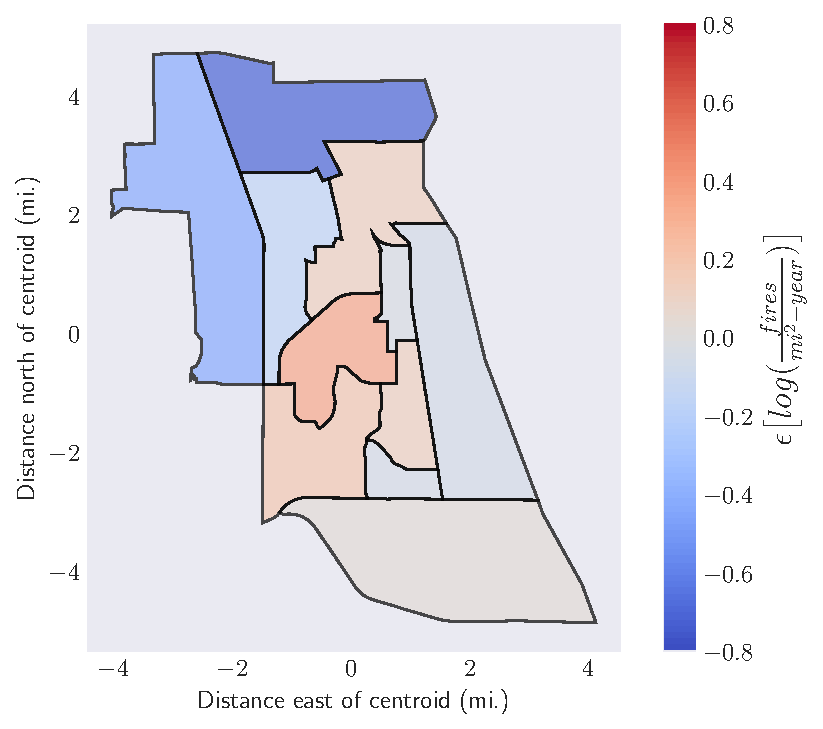
\includegraphics[width=.75\textwidth]{figures/spatial_correlation.pdf}
\caption{An example of a department that exhibits spatially correlated residuals. The hierarchical Poisson regression model appears to overpredict the fire count density rate in the northwestern census tracts and underpredict in the central census tracts. The fact that the residuals are similar for neighboring census tracts suggests that there are chronic factors that elevate or decrease the residential fire risk relative to the model's prediction.}
\label{fig:spatialcorr}
\end{figure}

Specifically Nadaraya-Watson\cite{nadaraya1964estimating} Kernel regression is performed on the residuals of the hierarchical Poisson model in order to generate improved estimates of $\Lambda_{i,j}$. This is a non-parametric statistical technique that is capable of learning non-linear functions. The idea is that the value of a function at a point can be estimated as a weighted average of the observed ``noisy" data points.  The weights are based on a kernel function, which gives observed data near the point of interest more weight than those that are far away. Though a Gaussian kernel (equation \ref{eqn:gaussian_kernel}) is used here, this method is different from the kernel density estimation described in section \ref{sec:kde} because the goal here is to estimate a function defined for each census tract, rather than to estimate a continuous density map given a set of observed incident locations. The updated estimate for the fire count density rate ($\hat{\lambda}^{\text{SR}}_{i,j}$) with smoothed residuals is calculated according to equation \ref{eqn:smooth_residual}:

\begin{equation}
  \label{eqn:smooth_residual}
  log(\hat\Lambda^{\text{SR}}_{i,j}) = log(\hat\lambda^{\text{HPR}}_{i,j}) + \tilde{\varepsilon}_{i,j}
\end{equation}

\noindent where $\tilde{\varepsilon}_{i,j}$ is the kernel smoothed residual function evaluated for census tract i,j. It is calculated according to equation \ref{eqn:smoother}:

\begin{equation}
  \label{eqn:smoother}
  \tilde{\varepsilon}_{i,j} = \sum_{k=1}^{N_i} H_{i,j,k}\varepsilon_{i,k}
\end{equation}

\noindent where $H_i$ is a smoothing matrix for department $i$. Note that equation \ref{eqn:smoother} is equivalent to $\tilde{\varepsilon}_{i} = H_{i}\varepsilon_{i}$. The smoothing matrix is calculated according to equation \ref{eqn:smooth_mat}.

\begin{equation}
  \label{eqn:smooth_mat}
  H_{i,j,k} = \frac{K(\textbf{x}_j,\textbf{x}_k)}{\sum_{n=1}^{N_i}K(\textbf{x}_j,\textbf{x}_n)}
\end{equation}

\noindent In other words, element $j$,$k$ of the smoothing matrix for department $i$ quantifies the amount of weight to put on the (noisy) observation from census tract $k$ to inform the estimation of the true value from census tract $j$. The denominator imposes the restriction that the sum of the weights from all $N_i$ tracts must sum to one. $K(\textbf{x}_j, \textbf{x}_k)$ is the Gaussian kernel function repeated in equation \ref{eqn:gaussian_kernel2}.

\begin{equation}
  \label{eqn:gaussian_kernel2}
 K(\textbf{x}_j, \textbf{x}_k) = \frac{1}{2\pi b^2}exp\bigg(\frac{-d^2(\textbf{x}_j,\textbf{x}_{k})}{2b^2}\bigg)
\end{equation}

The distance function, $d(\textbf{x}_j,\textbf{x}_{k})$, between tract $j$ and tract $k$, is less straightforward here than it was in the kernel density estimation of section \ref{sec:kde}. One may think to use a euclidean distance between the centroids of census tracts, but this approach unduly weights small census tracts over larger ones because the distance between a tract's centroid to its boundary is generally larger for larger census tracts. Instead, a method of calculating $d(\textbf{x}_j,\textbf{x}_{k})$ that is invariant to the census tract size is presented here. The idea is to make the distances between tracts based on degrees of neighborship rather than a euclidean distance. It is described in equation \ref{eqn:degreeofsep}. 


\begin{equation}
  \label{eqn:degreeofsep} 
  d(\textbf{x}_j,\textbf{x}_{k}) = 
  \begin{cases} 
      0 & \text{if } j=k \\
      1 & \text{if tract \textit{j} touches tract \textit{k}} \\
      2 & \text{if tract \textit{j} touches a tract that touches tract \textit{k}} \\
      ... & ... \\     
   \end{cases}
\
\end{equation}

An example of the resulting distance matrix is shown for a department in equation \ref{fig:distance_mat}. 

  \begin{figure}[!htb]
       \begin{center}
  %
          \subfloat[Layout of census tracts]{%
              \label{fig:tract_layout} 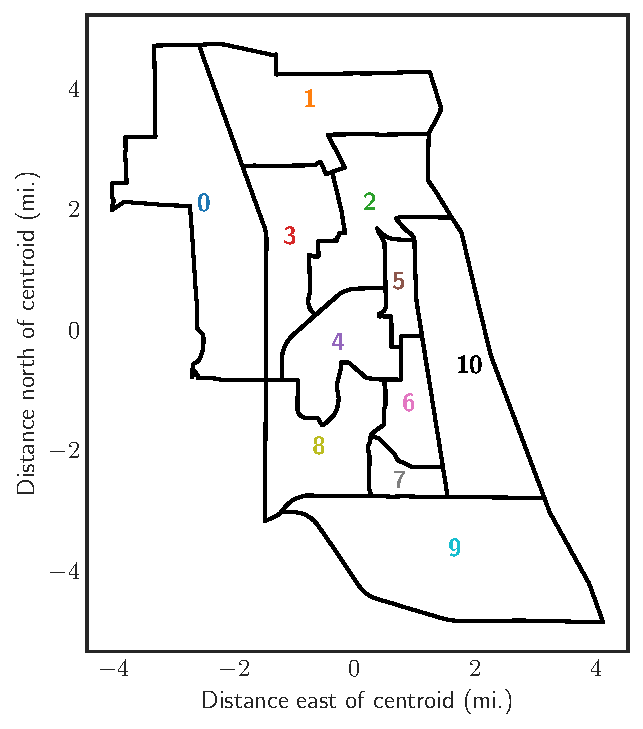
\includegraphics[width=.4\textwidth,keepaspectratio]{figures/tract_num.pdf}
          }%
          \subfloat[Distance matrix based on neighborship]{%
             \label{fig:distance_mat} 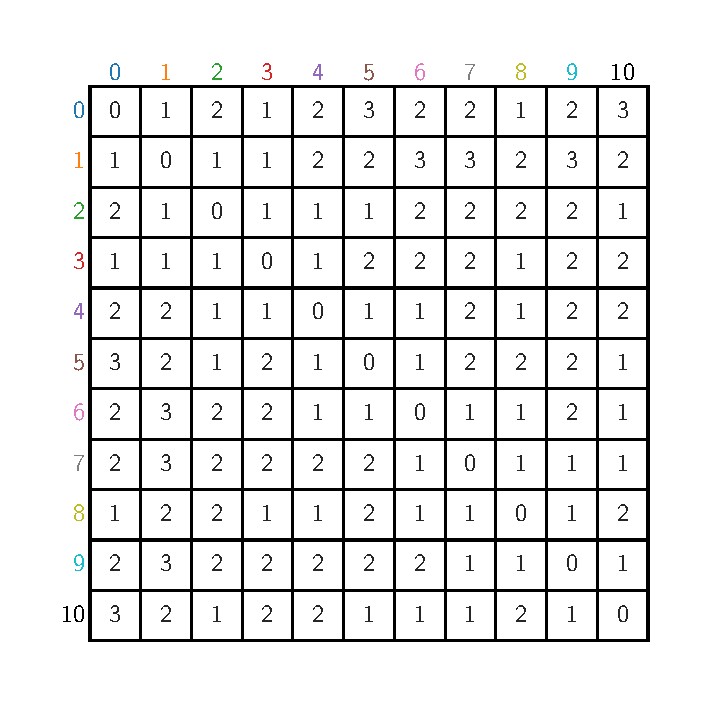
\includegraphics[width=.45\textwidth,keepaspectratio]{figures/sep_matrix.pdf}
          } %           
      \end{center}
      \caption{An example of the resulting distance matrix for a department}
     \label{fig:sep_example}
  \end{figure}
  
  
  With this approach, the bandwidth $b$ is set to one for all departments because the length scale associated with the spatial factors of interest is assumed to be one degree of neighborship. 
 
 
 \section{Model evaluation and comparison}
 The naive count model described in section \ref{countmodel} serves as the performance baseline for all other models described in this paper. The RMSE (equation \ref{eqn:deviance}) for this model is 7.61 fires. The comparison of the models against each other is shown in table \ref{table:dev_table}. 

    \begin{table}[htb] \centering
    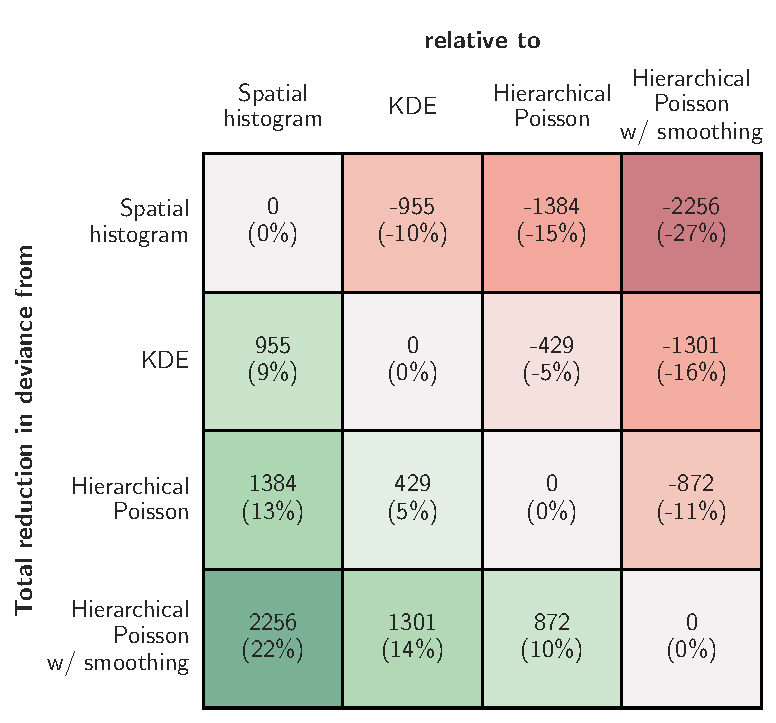
\includegraphics[width=.75\textwidth]{figures/dev_table.pdf}
    \caption{A comparison of the RMSE of 5-year forecasts between all models. The model corresponding to the row is compared against the model corresponding to the column. For example, the green cell in the bottom left indicates that the hierarchical Poisson model with kernel smoothing had total RMSE that is 1.41 fires smaller than the spatial histogram model of section \protect\ref{countmodel}, which is a 19\% improvement.}
    \label{table:dev_table}
    \end{table}
  
    \begin{table}[htb] \centering
    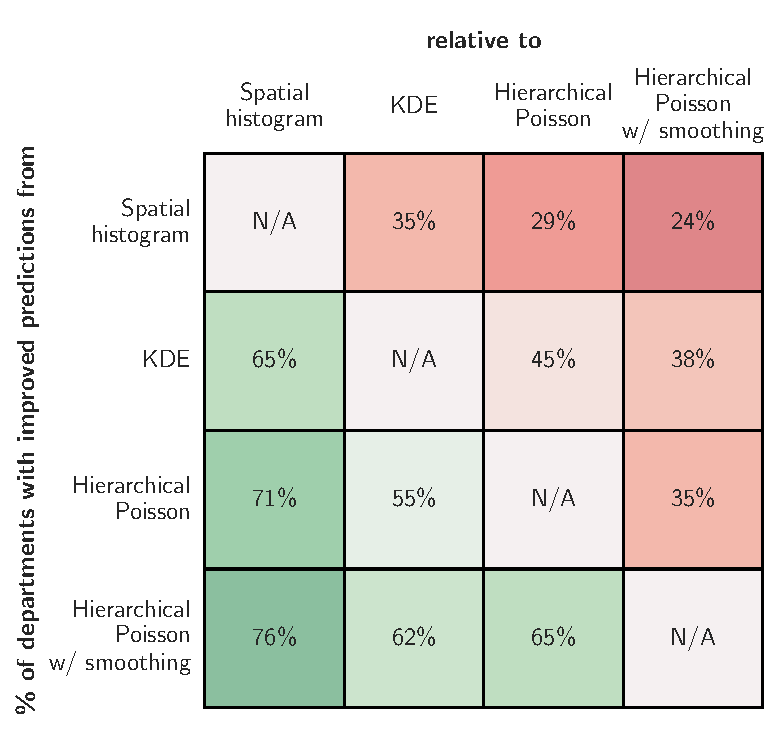
\includegraphics[width=.75\textwidth]{figures/department_comparison.pdf}
    \caption{A comparison of the number of department with improved predictions from the model corresponding to the row relative to the model corresponding to the column.}
    \label{table:dep_comparison}
    \end{table}
    
    
    The spatial histogram model performed the worst of the models, which is not surprising given that it is the simplest. The integrated kernel density approach led to a 7\% reduction in total RMSE relative to the spatial histogram model. This is likely due to the fact that fire risk factors spread across census tract boundaries. One can imagine a scenario in which two census tracts neighbor each other and during training interval, several fires occur near the boundary separating these tracts, but by chance, most of these fires occur in one of the tracts. The housing units near the boundary in the tract with fewer fires is likely still at an elevated residential fire risk due to proximity to these past fires. This assumption is incorporated into the KDE approach, but not the spatial histogram approach. Also, as previously stated, the spatial histogram can be viewed as a special case of the KDE approach in which the bandwidth is set to zero. It is therefore not surprising that a statistically optimized bandwidth would yield better predictions than one that is arbitrarily set. 
    
    The hierarchical Poisson regression model outperforms both of the purely spatial models illustrating the utility of incorporating structural and sociodemographic information into the model. This model has the attribute that census tracts with the same structural and sociodemographic profile in the same department receive the same 5-year predictions. This is advantageous because one census tract may experience an abnormally large or small number of fires during the training interval, which would skew the predictions of both the spatial histogram and the integrated KDE approach. However, the hierarchical Poisson model is more robust because it is able to learn from the observations in demographically similar tracts. Finally, the kernel smoother on top of the hierarchical Poisson predictions led to a an 6\% reduction in RMSE. The choice of the bandwidth and smoothing matrix is key here; if a euclidean distance with a small bandwidth is chosen, the predictions from this model will be the same as those from the spatial histogram. The use of the distance matrix that is invariant to census tract size performs well here. This is likely because spatially correlated residuals are the product of fire risk factors that are not included in the regression model or modeling misfit of neighboring tracts that are demographically similar. Regardless of the cause, if the model's estimation of the fire count density rate is higher or lower for a group of neighboring census tracts, it is likely to make similar errors on the test data. 
    
    Another figure of merit for comparing models is the percentage of departments whose  5-year forecasts are improved (i.e. lower RMSE) from the use of one model over another. These results are shown in table \ref{table:dep_comparison}. The trends are similar to those in table \ref{table:dev_table}.
    

    
  
  \section{Conclusions}
  This work highlights the utility of combining both spatial and socio-demographic information into a model for predicting residential fire counts at the census tract level. The kernel density estimation approach with bandwidth parameters optimized from 5-fold cross validation generated 5-year forecasts that had a 7\% lower RMSE than a naive ``spatial histogram" model, which simply uses the observed rate of past fires to predict future fire counts. An inverse correlation was found between the optimized bandwidth from KDE and the average population of the department's covered census tracts. This suggests that fire risk factors spatially vary over smaller length scales for departments with higher average population densities. An examination of the features revealed a nearly linear relationship between fire density rate and population density across both rural and urban census tracts. Factors associated socioeconomic disadvantage (i.e. race, income, education) were shown to affect the fire rate per person. Furthermore, a high fraction of housing units built before 1950 was also shown to increase the fire rate per person. A high fraction of vacant housing units was also found to increase this quantity as well. The understanding of these risk factors was used to inform the design of a Bayesian hierarchical Poisson regression model, which identifies a relationship between population density and fire count density for all departments, but allows each department to have its own effect for the demographic and structural attributes. The predictions from this model showed a 13\% improvement relative to the naive count model. Finally, An examination of the residuals of the regression model revealed spatial correlation. This means that there are cases where the regression model overpredicts or underpredicts the fire counts for groups of neighboring census tracts. In these cases, there are likely chronic factors that influence fire risk in these regions that are not accounted for in the regression model. Even though they are not specifically identified, the use of kernel regression on the residuals allows the model to incorporate these factors indirectly to make even more improved predictions. The final model exhibited a 19\% improvement to the RMSE relative to the naive count model. 

  
 \appendix
 

\section{Dispersion considerations}
\label{dispersion}
  \begin{figure}[htb] \centering
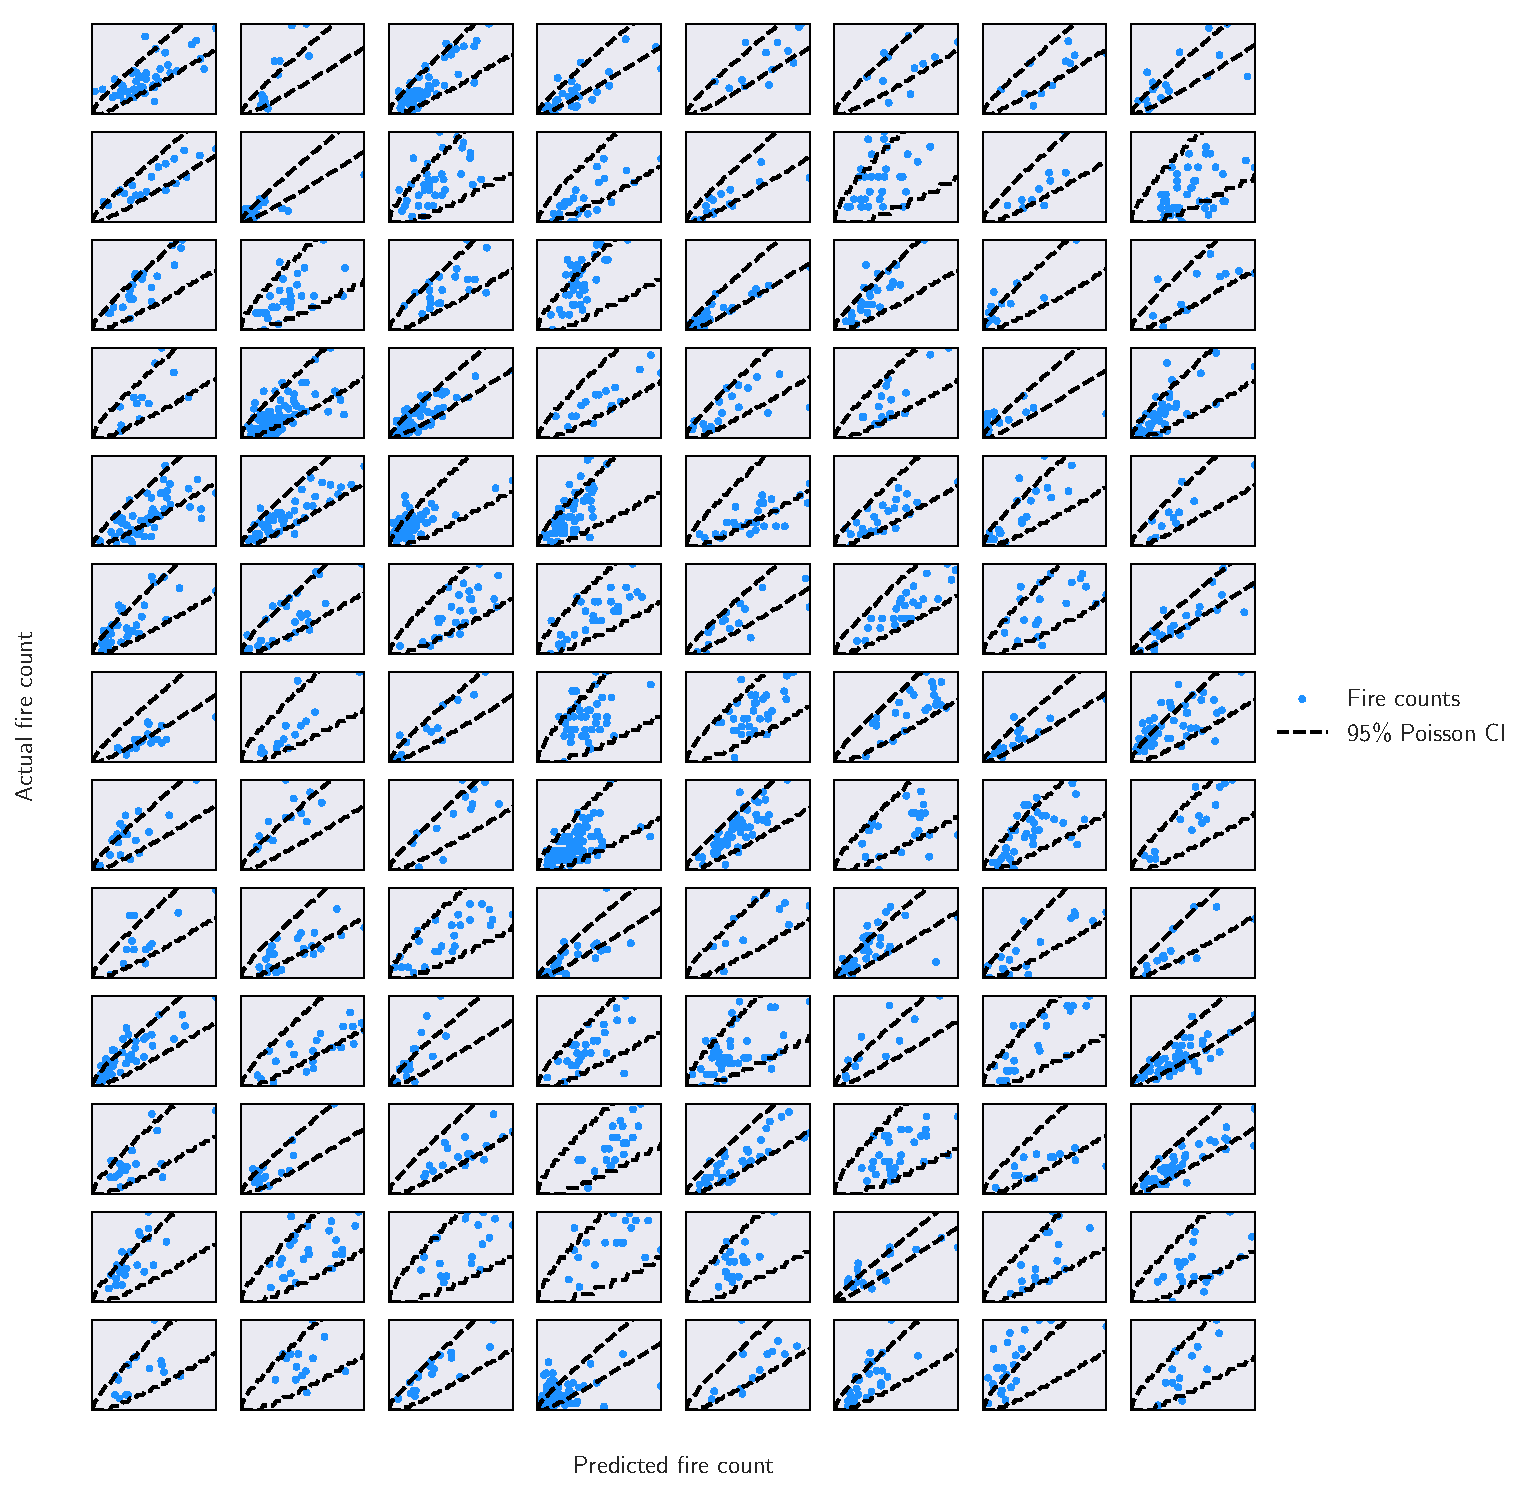
\includegraphics[width=1\textwidth]{figures/dispersion.pdf}
\caption{Depiction of the number of fires that occurred during the test interval vs. the expected number of fires from the hierarchical Poisson regression model with smoothing, which is the best estimate of the mean rate of fires for each census tract. The dashed line represents a 95\% confidence interval for a Poisson distribution centered around the expected fire count. This indicates that the fire counts are not significantly overdispersed over a five year period for most departments in the dataset.}
\label{fig:dispersion}
\end{figure}
\clearpage
\bibliographystyle{unsrtnat}
\bibliography{./references.bib}
\end{document}
